\documentclass[11pt]{article}
\usepackage[T1]{fontenc}
\usepackage[english]{babel}
\usepackage{fullpage}
\usepackage{graphicx}
\usepackage{caption}
\usepackage{subcaption}
\newcommand{\HRule}{\rule{\linewidth}{0.5mm}}
%\def\wl{\par \vspace{\baselineskip}}

\begin{document}

% TITLE PAGE
\begin{titlepage}
\begin{center}

% Header
\textsc{\LARGE AA241X: Design, Construction, and Testing of Autonomous Aircraft}\\
\HRule \\[0.4cm]

\includegraphics[width=1.0\textwidth]{./skynet}~\\
\HRule \\[0.4cm]
\textsc{\Large Final Report}\\
{\large \today}
\vfill

% Authors
\begin{minipage}{0.4\textwidth}
\begin{flushleft} \large
\emph{Authors:}\\[0.5cm]
Kartikey Asthana\\
\texttt{kasthana@stanford.edu}\\[0.5cm]
Peter Blake\\
\texttt{psblake@stanford.edu}\\[0.5cm]
Brandon Jennings\\
\texttt{bjennin@stanford.edu}\\[0.5cm]
Erik Moon\\
\texttt{emoon1@stanford.edu}\\[0.5cm]
Sravya Nimmagadda\\
\texttt{sravya@stanford.edu}\\[0.5cm]
Akshay Subramaniam\\
\texttt{akshays@stanford.edu}\\[0.5cm]
Ian Villa\\
\texttt{ianvilla@stanford.edu}\\[0.5cm]
Jerry Watkins\\
\texttt{watkins2@stanford.edu}\\[0.5cm]
\end{flushleft}
\end{minipage}
\begin{minipage}{0.4\textwidth}
\begin{flushright} \large
\emph{Degree \& Department:} \\[0.5cm]
Ph.D. Candidate\\
Aeronautics \& Astronautics\\[0.5cm]
M.S. Candidate\\
Graduate School of Business\\[0.5cm]
M.S. Candidate\\
Mechanical Engineering\\[0.5cm]
M.S. Candidate\\
Graduate School of Business\\[0.5cm]
Ph.D. Candidate\\
Aeronautics \& Astronautics\\[0.5cm]
Ph.D. Candidate\\
Aeronautics \& Astronautics\\[0.5cm]
B.S. \& M.S. Candidate\\
Aeronautics \& Astronautics\\[0.5cm]
Ph.D. Candidate\\
Aeronautics \& Astronautics\\[0.5cm]
\end{flushright}
\end{minipage}
\end{center}
\end{titlepage}

% TABLE OF CONTENTS
\clearpage
\tableofcontents
\vfill
\clearpage

\section{Introduction}
\label{Introduction}
Since the early 2000's, Stanford Aeronautics and Astronautics has taught the AA 241X: Design, Construction and Testing of Autonomous Aircraft course with various missions over the years. In Spring of 2014, teams were tasked with developing an autonomous aircraft to search and accurately locate four targets within the perimeter of Lake Lagunita. Among these teams was Skynet, a group of eight individuals from different backgrounds and expertise who, throughout the ten weeks, collaborated to organize, design, test, and fly various aircraft, guidance, control, and mission systems to optimally complete the search and rescue. The following report outlines the team's structure, mission strategy, aerodynamic design, control strategy, fabrication accounts, flight test data, and overall competition performance.

\section{The Team}
\label{Team}
\subsection{Team Structure}
\label{TeamStrc}
\subsection{Team Communication \& Logistics}
\label{TeamCommLog}
In order to facilitate group discussions, a when2meet form was utilized online. Based on its results, the team met briefly after class on Mondays and Wednesdays for brief sub team status updates and coordination. Major team meetings were held on Fridays during the typical class time on the second floor of Durand and were spent discussing topics requiring everyone's attendance such as aircraft design and mission strategy.

The team also utilized online methods to meet communication needs. A Google Group was utilized for formalized notices and e-mail discussions. Short-form and quick information relays were handled by a GroupMe that could be accessed via phone or computer.

Data Storage and problem set completion was made possible via our Google Drive, Google Docs, and a Wordpress. All team data, code, and photos were uploaded into categorically defined folders in our Google Drive. Spreadsheets recording budget, weather data, contact information, useful links, and most importantly, problem set requirements were also held here. Having all of these documents in a single location and accessible by all of the team was the last step in facilitating good communication and ensured proper problem set completion. Once written, relevant text, data, graphs, and videos were uploaded to skynet241x.wordpress.com.

\section{Mission}
\label{Mission}
% KARTIKEY

\section{Airframe Design}
\label{Vehicle}

\subsection{Propulsion System Analysis}

The propulsion system analysis was performed in three parts:
\begin{enumerate}
\item Propeller analysis
\item Motor analysis
\item Propeller and Motor matching
\end{enumerate}

\subsubsection{Propeller Analysis}

For the propeller analysis, we used wind tunnel experimental data from the UIUC Propeller Data Site \footnote{http://aerospace.illinois.edu/m-selig/props/propDB.html}. The exact same propeller data was unavailable in the database, so we used a very similar propeller (Graupner CAM Slim 9x5) albeit from a different manufacturer.

The data was given in terms of the rotations per second instead of the angular velocity and hence, the following scaling had to be performed

\begin{eqnarray*}
\lambda &=& \frac{J}{\pi} \\
C_T &=& \left( \frac{2}{3} \right)^3 C_T ^ \prime \\
C_P &=& \frac{1}{\pi} \left( \frac{2}{3} \right)^3 C_P ^ \prime \\
\eta &=& \eta ^ \prime
\end{eqnarray*}
where $\lambda$ is the advance ratio based on the angular velocity, $J$ is the advance ratio based on the rotations per second, $C_T$ is the thrust coefficient, $C_P$ is the power coefficient and $\eta$ is the propeller efficiency. The primed quantities are the ones reported in the database.

\subsubsection{Motor Analysis}
The motor analysis was performed by using the standard electric motor model. The motor speed constant, motor resistance and the no-load motor current were obtained from experimentally measured values on the manufacturer's website \footnote{http://www.maxxprod.com/pdf/HC2808-xxxx.pdf}.

The values of the model constants are reported below:
\begin{eqnarray*}
K_v &=& 980 \left( \frac{2 \pi}{60} \right) \; rad/s/volt \\
R_m &=& 0.220 \; \Omega \\
i_0 &=& 0.4 \; A
\end{eqnarray*}

\subsubsection{Propeller and Motor Matching}
For a given free-stream velocity, the required torque for the propeller was calculated as a function of the angular velocity of the propeller. For the motor, the torque generated was calculated as a function of the angular velocity. By matching these two torques, we solved for the angular velocity and obtained the total propulsive efficiency. This process is illustrated in Figure~\ref{fig:prop-motor1}.
\begin{figure}[h!]
  \centering
    \begin{subfigure}[b]{0.49\textwidth}
                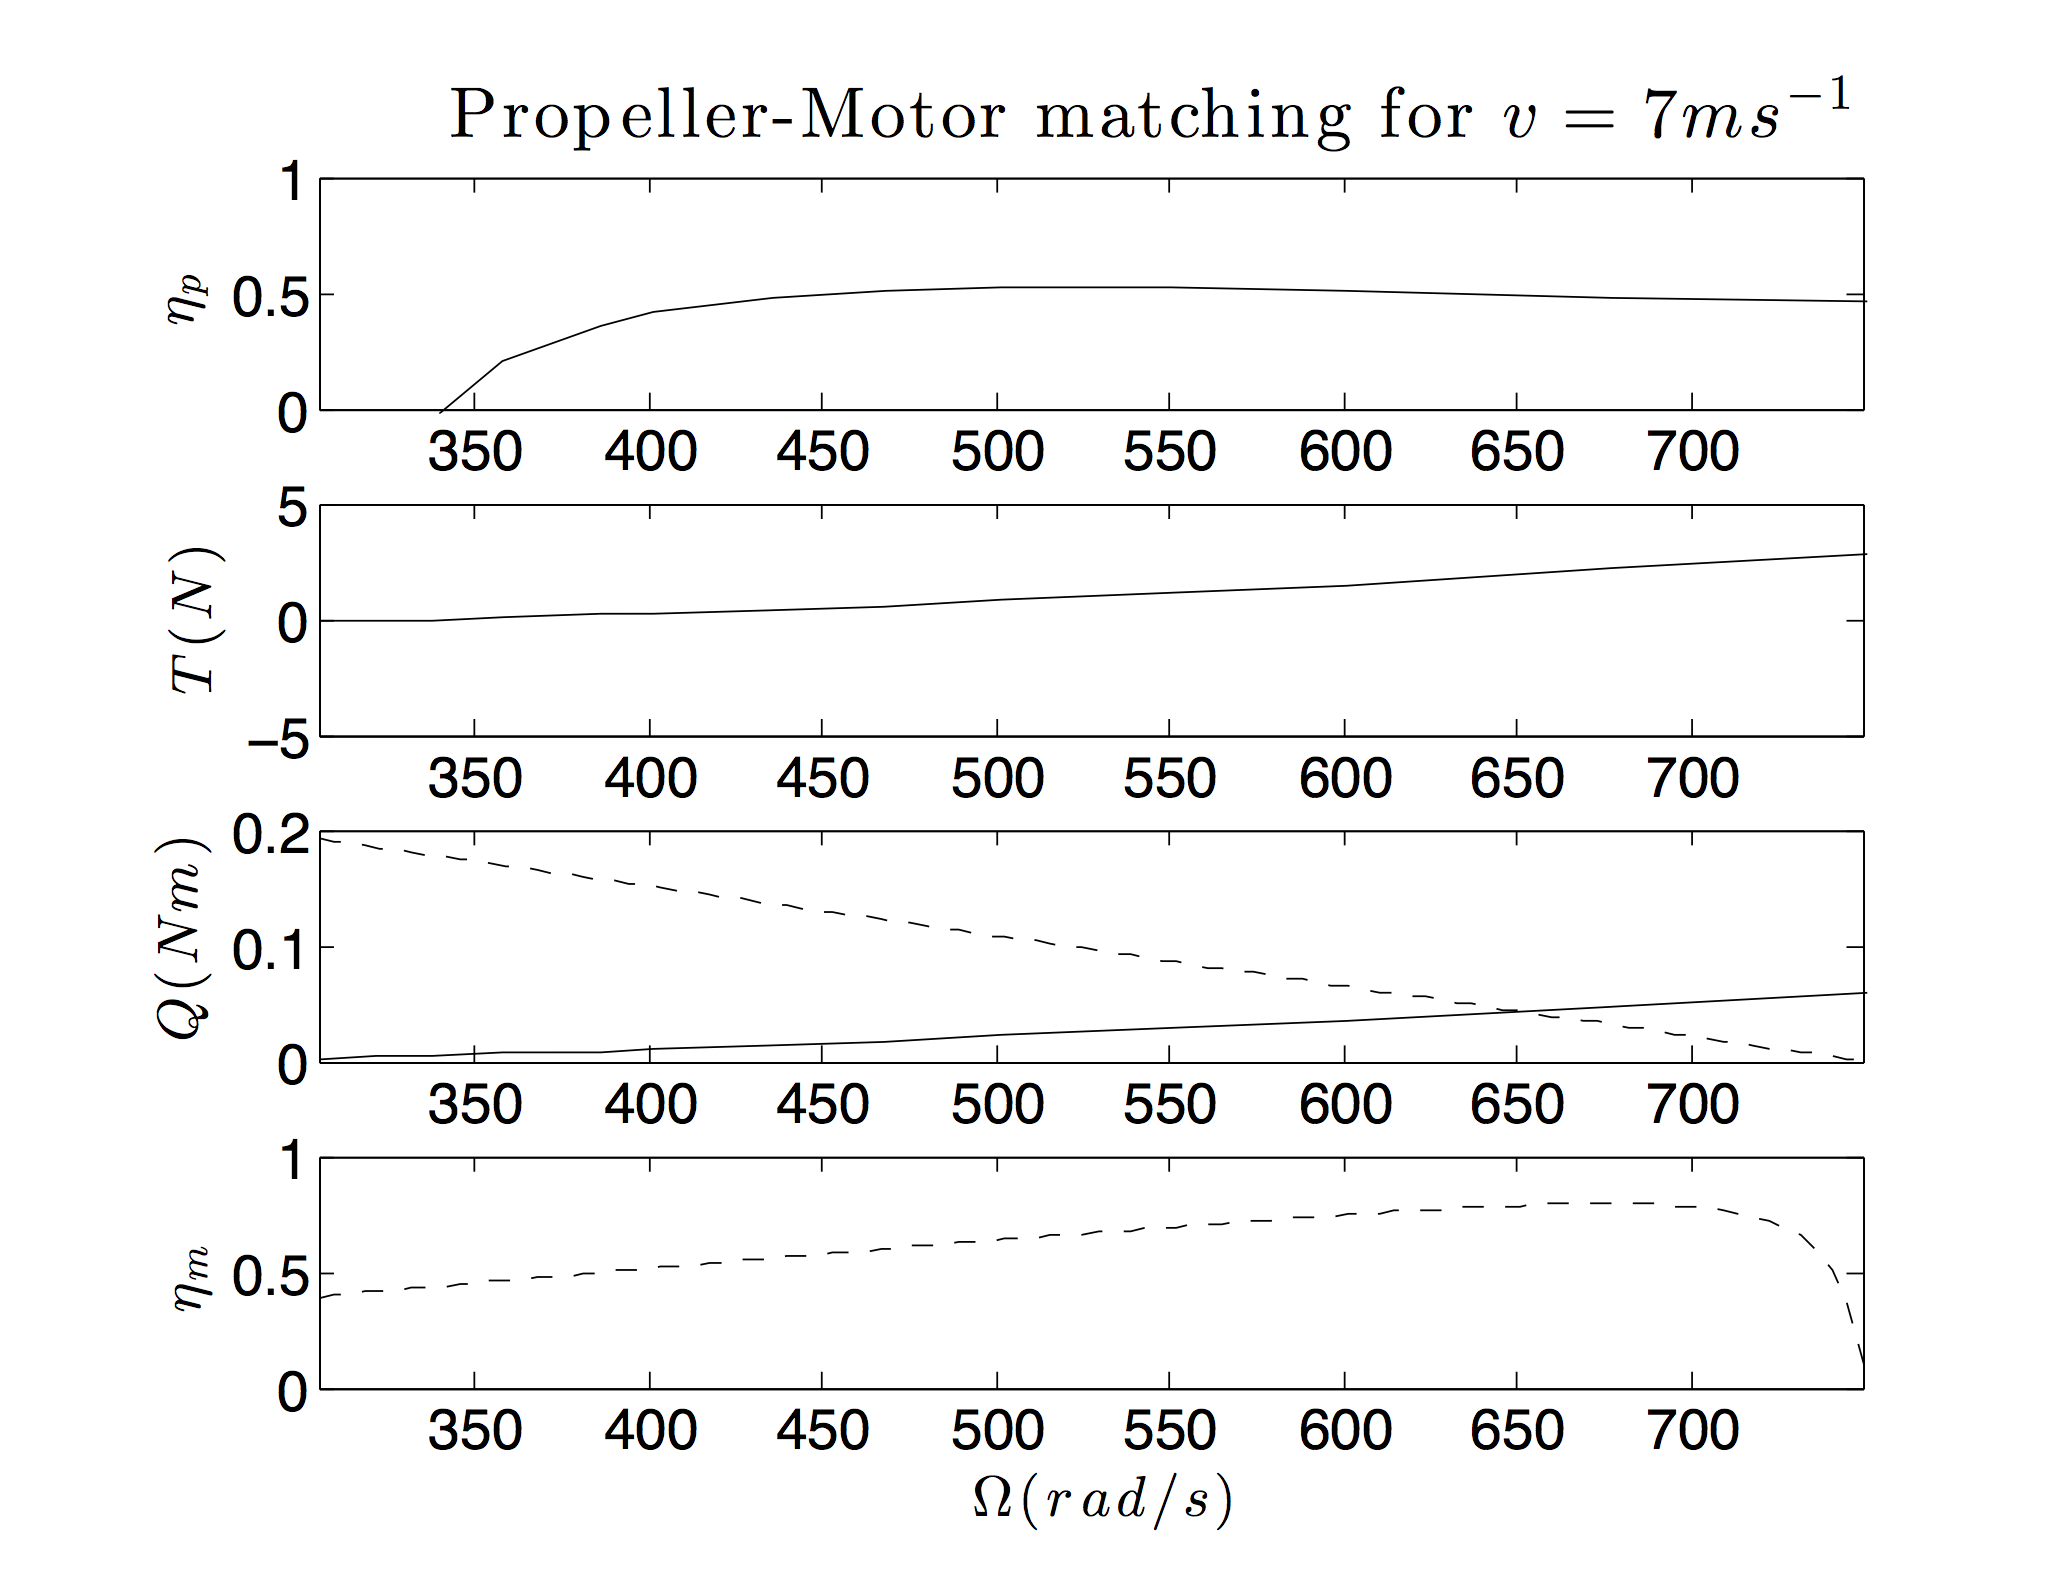
\includegraphics[width=\textwidth]{Figures/PS3/propmotor_v07p0.png}
                \caption{$v = 7 \; m/s$}
        \end{subfigure}
        \begin{subfigure}[b]{0.49\textwidth}
                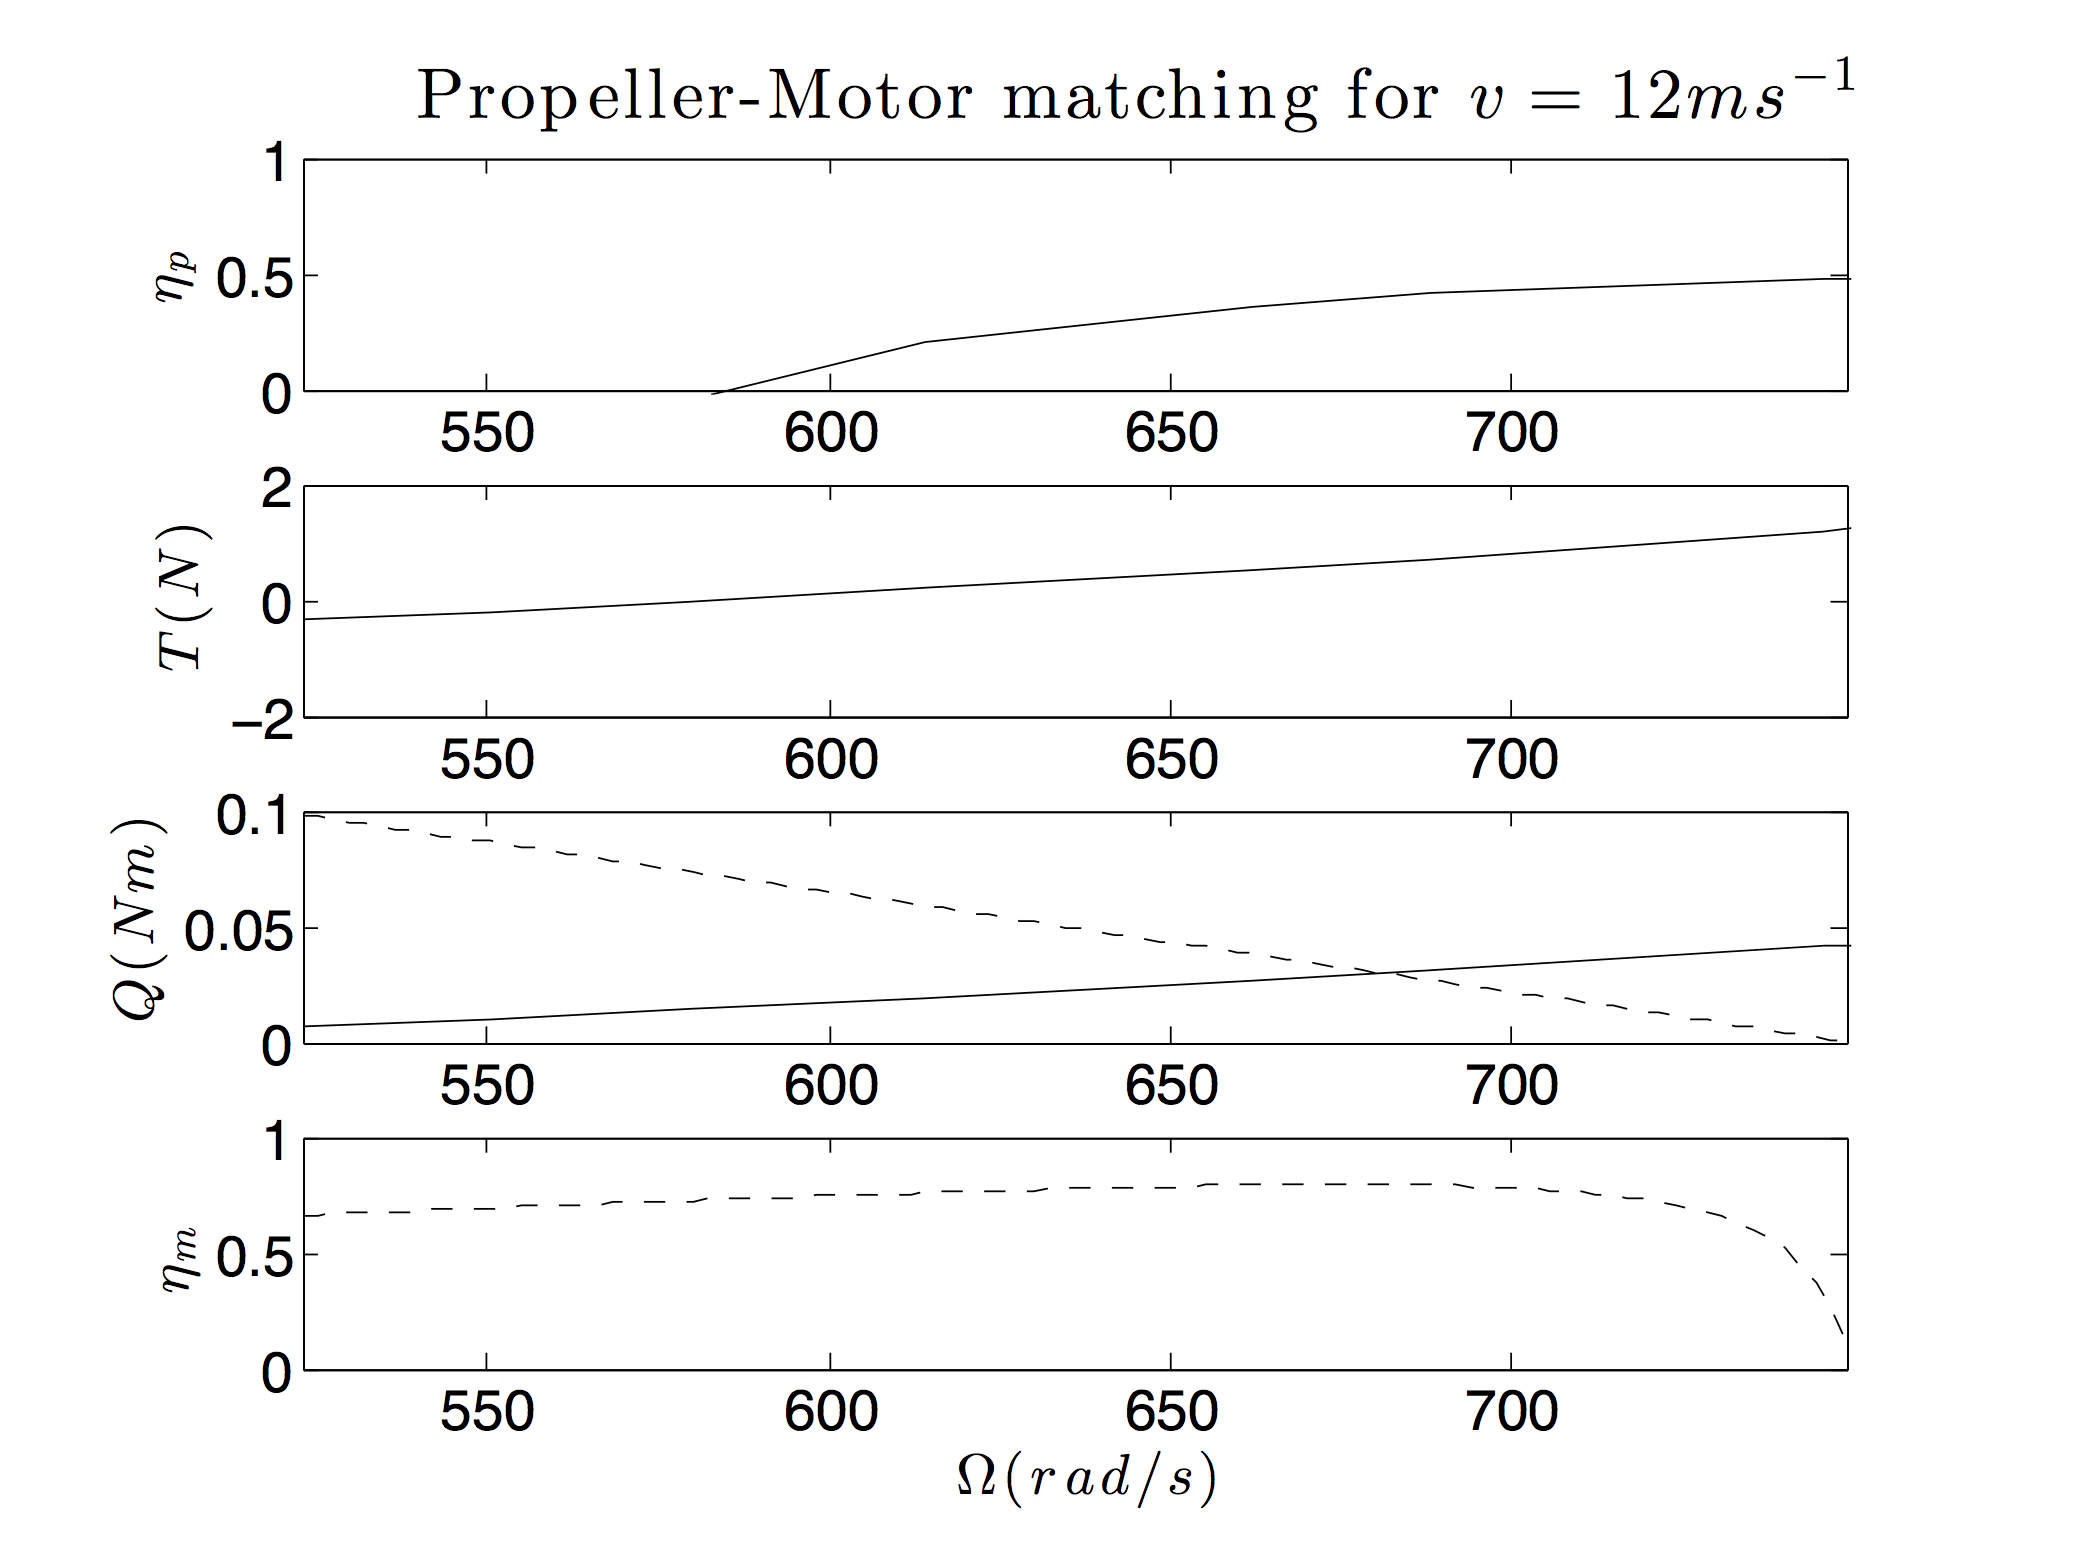
\includegraphics[width=\textwidth]{Figures/PS3/propmotor_v12p0.png}
                \caption{$v = 12 \; m/s$}
        \end{subfigure}%
  \caption{Propeller-Motor matching shown graphically. Solid lines: propeller curves. Dashed lines: Motor curves}\label{fig:prop-motor1}
\end{figure}

For the $7 \; ms^{-1}$ case, we see that the propeller efficiency, $\eta_p$ peaks at very low angular velocities and hence the total propulsive efficiency is poor. For the $12 \; ms^{-1}$ case, the propeller efficiency, $\eta_p$ peaks at high angular velocities which again leads to a low total propulsive efficiency. Optimizing the total propulsive efficiency over different airspeeds, we get the best motor-propeller matching illustrated in Figure~\ref{fig:prop-motor2}

\begin{figure}[h!]
  \centering
  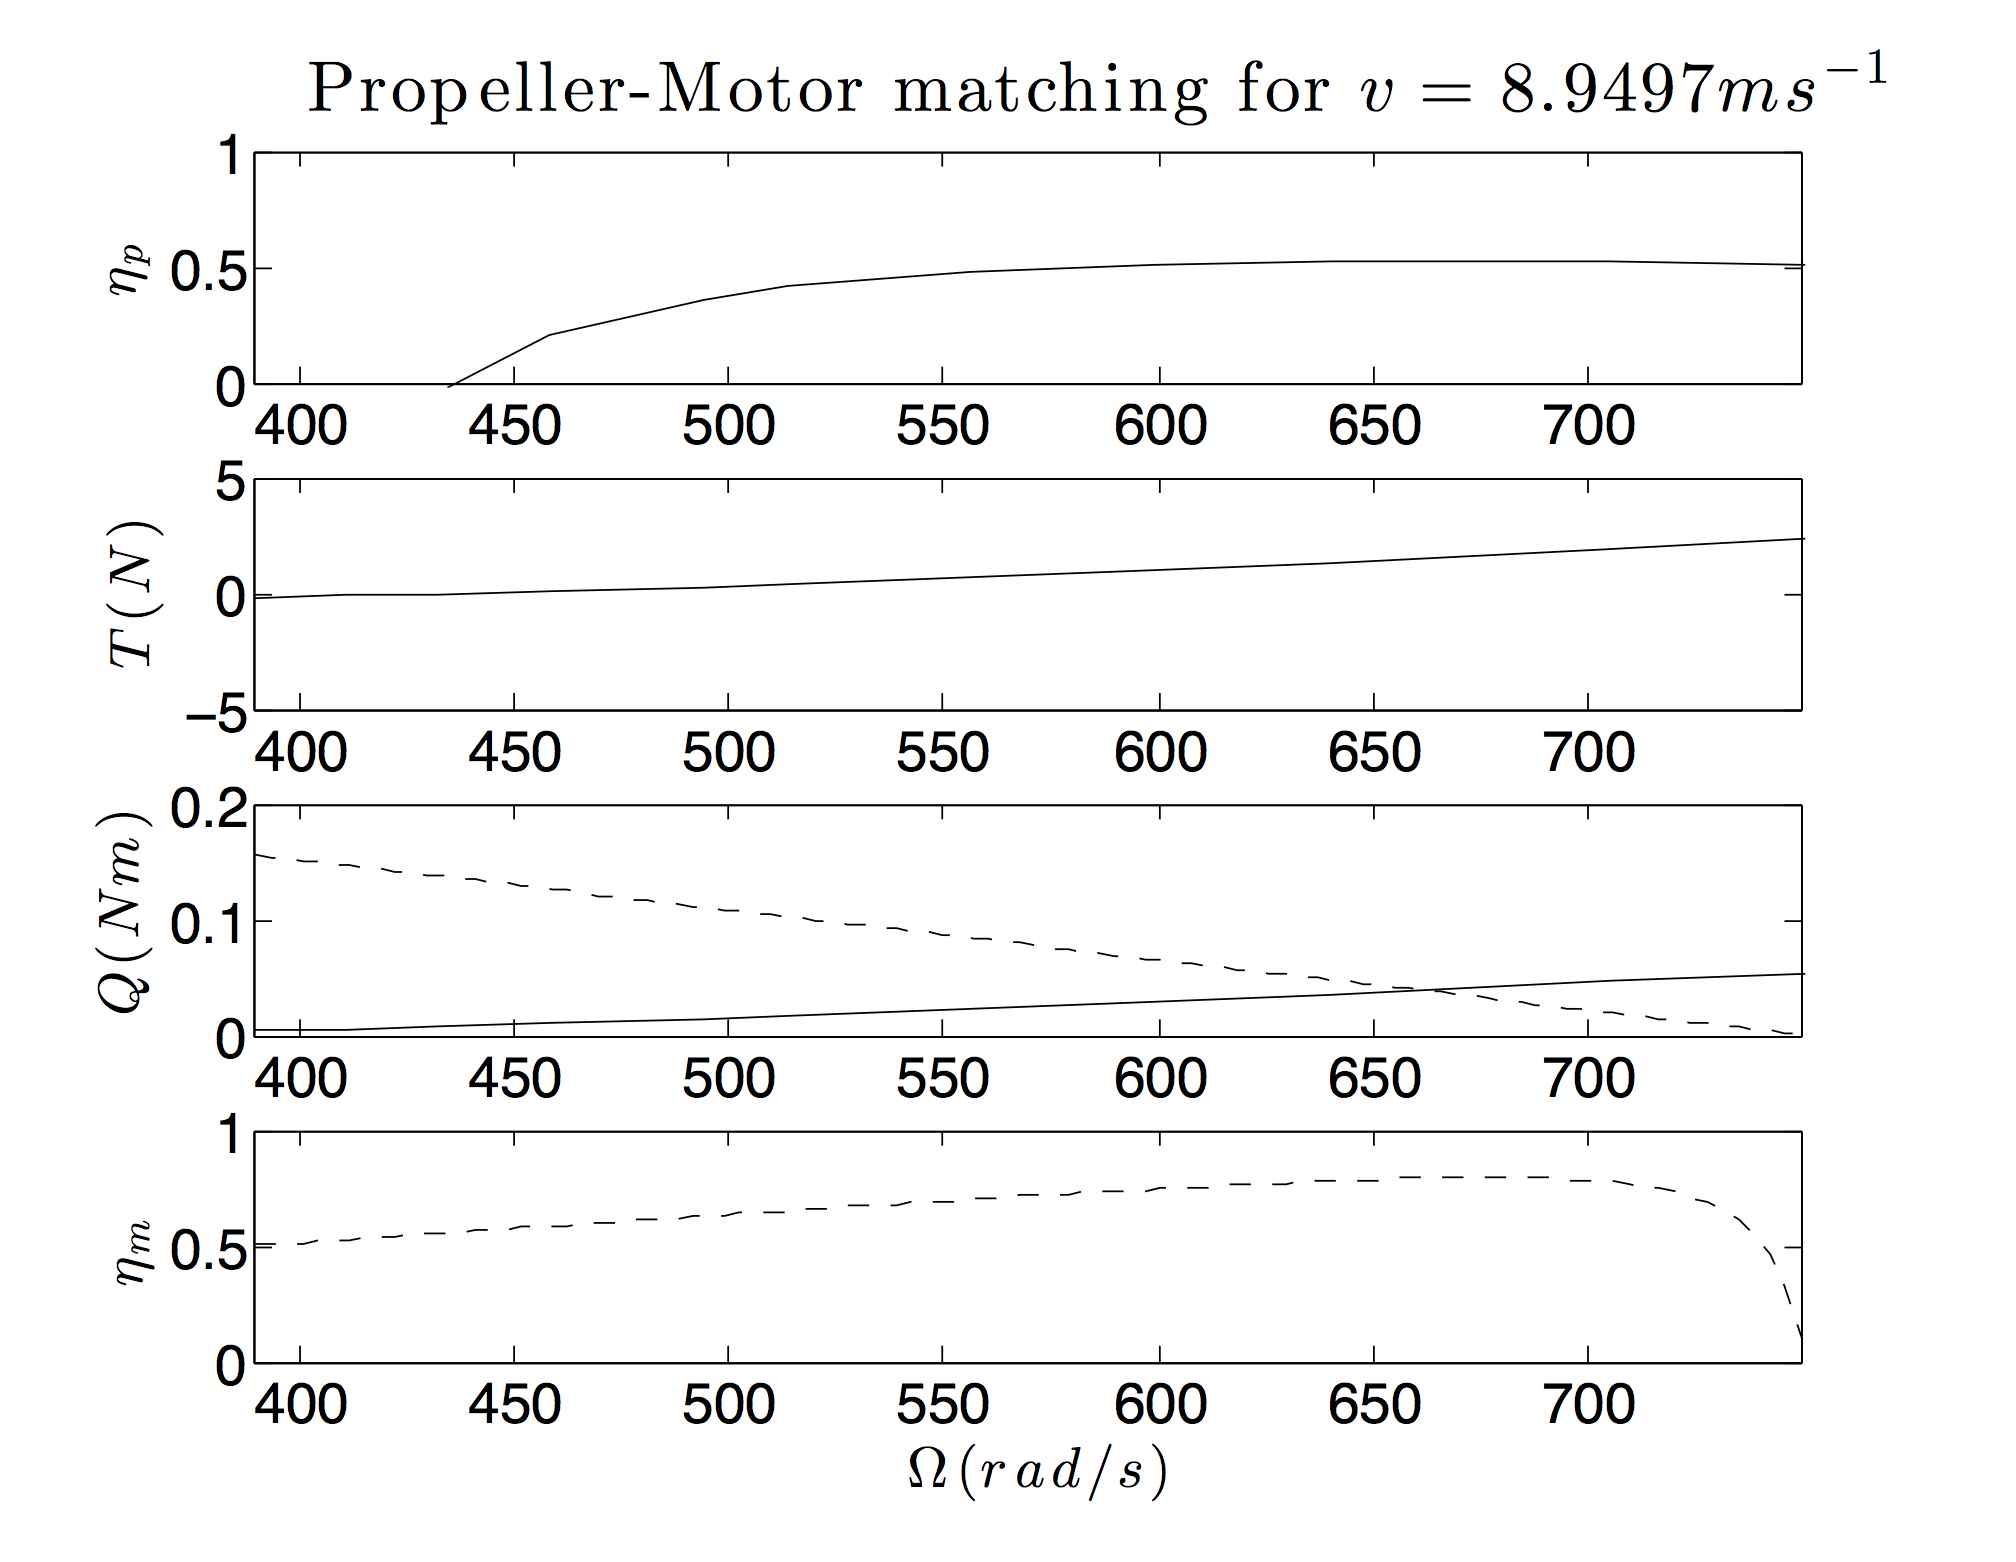
\includegraphics[width=\textwidth]{Figures/PS3/propmotor_opt.png}
  \caption{Optimal Propeller-Motor matching shown graphically. Solid lines: propeller curves. Dashed lines: Motor curves}\label{fig:prop-motor2}
\end{figure}

The total propulsive efficiency and the thrust are plotted against airspeed in Figure~\ref{fig:teff-thrust}.

\begin{figure}[h!]
  \centering
    \begin{subfigure}[b]{0.49\textwidth}
                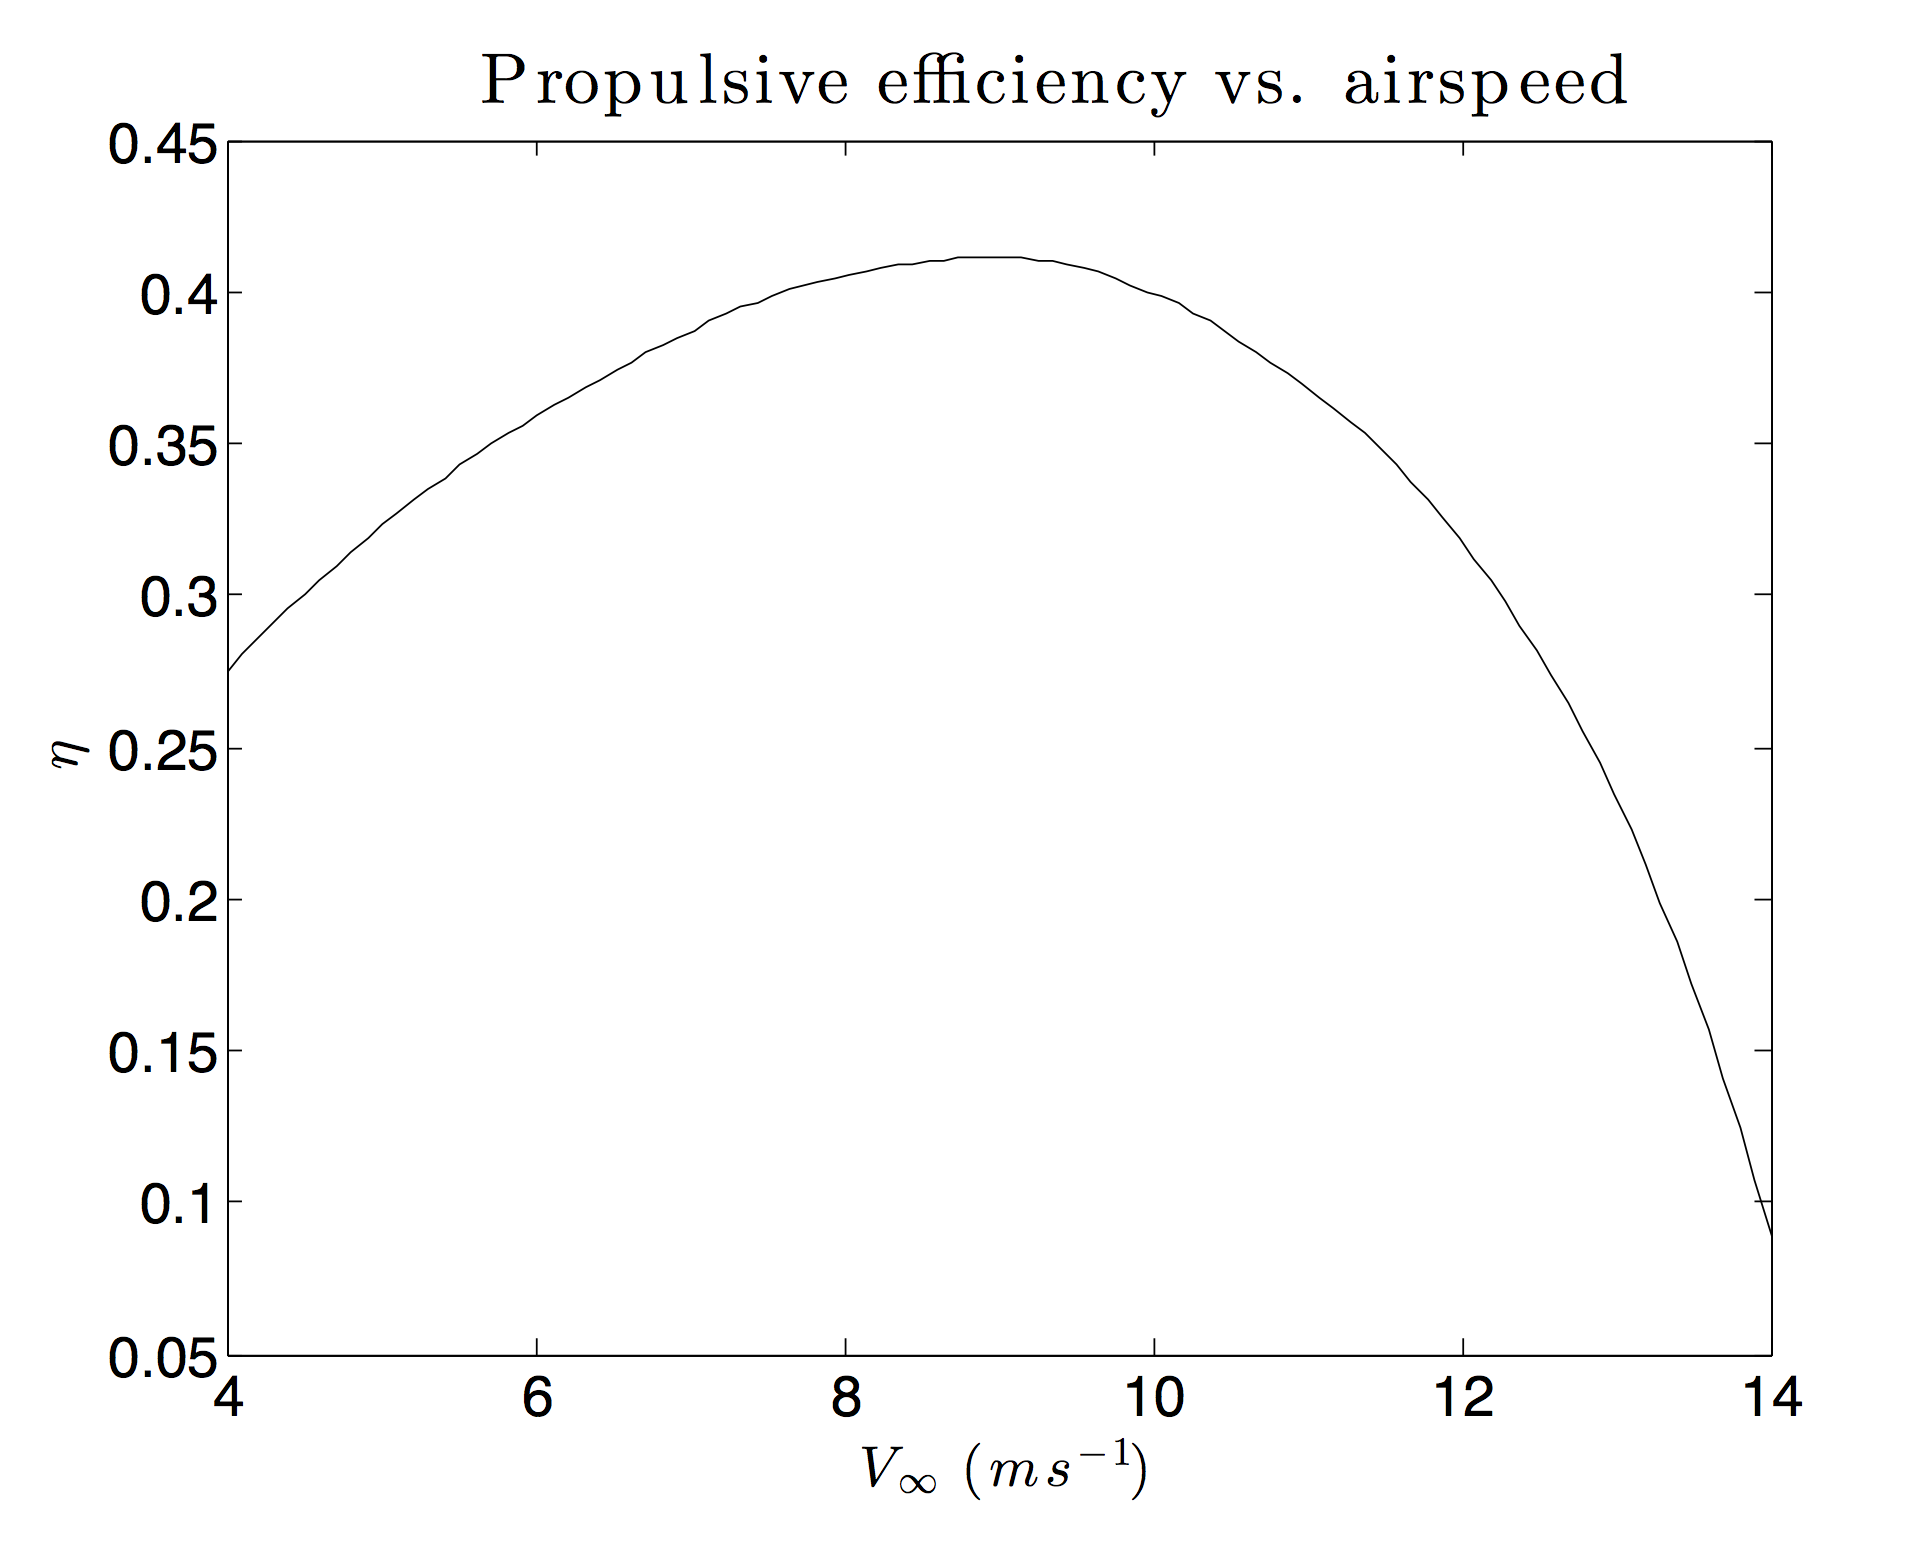
\includegraphics[width=\textwidth]{Figures/PS3/Teff.png}
                \caption{Plot of the total propulsive efficiency against airspeed}
        \end{subfigure}
        \begin{subfigure}[b]{0.49\textwidth}
                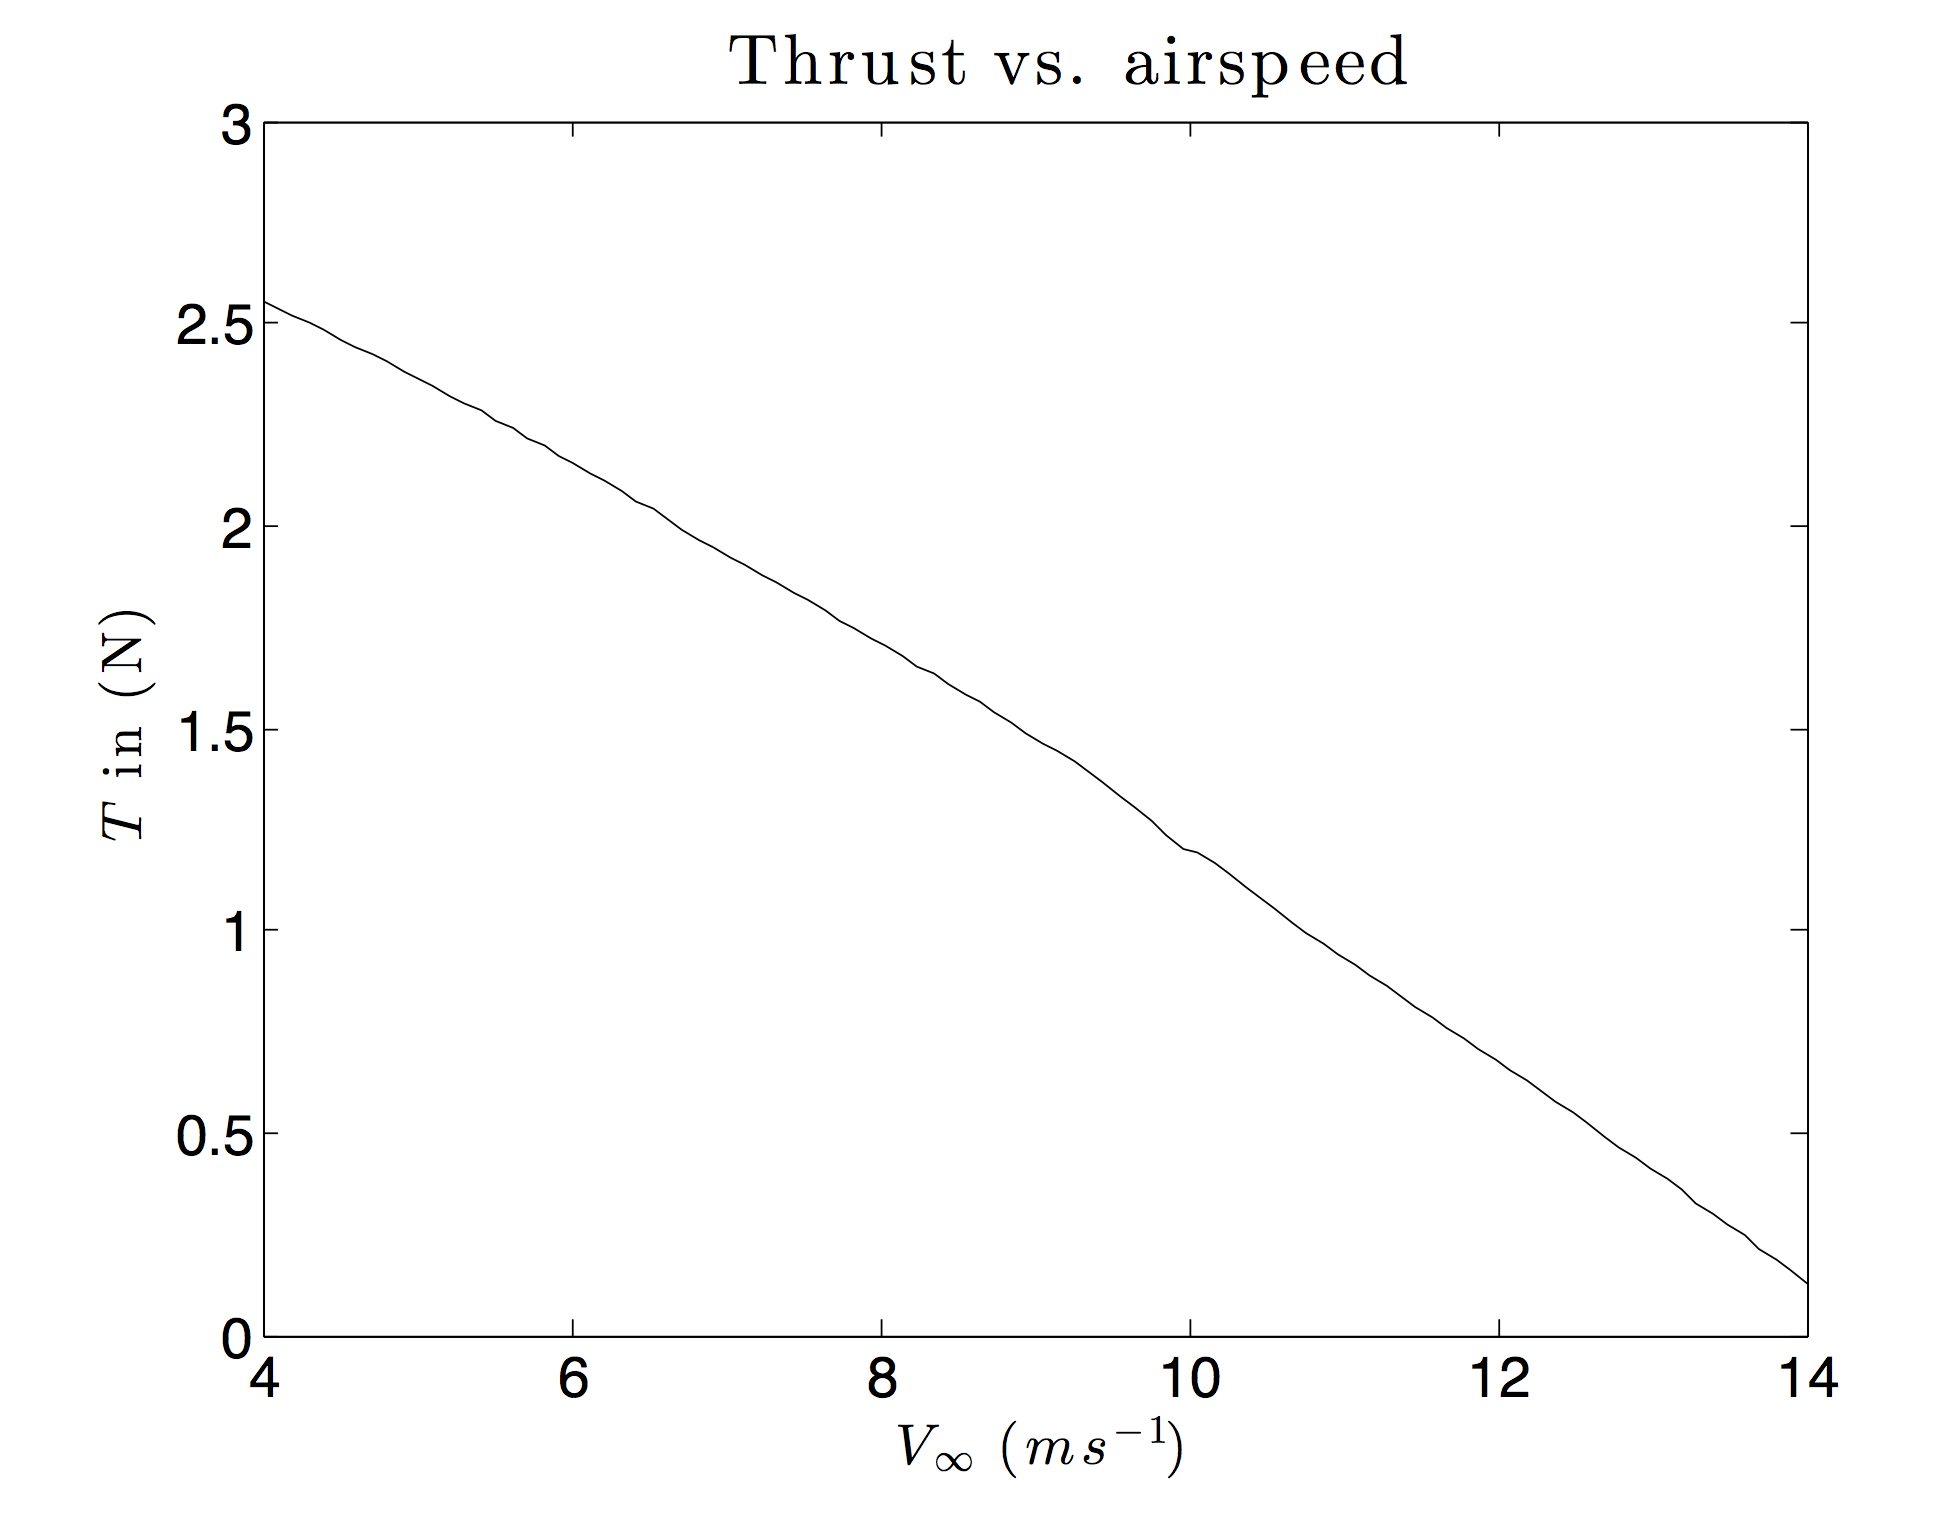
\includegraphics[width=\textwidth]{Figures/PS3/Thrust.png}
                \caption{Plot of the total thrust against airspeed}
        \end{subfigure}%
  \caption{Thrust and efficiency plots}\label{fig:teff-thrust}
\end{figure}

\subsection{Design Approach}
\label{DsignAppr}

For our mission plan, it is critical that we climb to an altitude of $400 ft$ as fast as we can to efficiently scout the search area and sight all four targets as soon as we can. Hence, the rate of climb for our airplane is of crucial importance. In addition to this, the endurance of our aircraft is also very important since the allowed battery consumption is very limiting. We designed our aircraft mainly based on these two considerations.

First, we obtained the drag polar for a generic 2D semi-symmetrical airfoil section (Clark-Y) in XFLR5 that we used as our first estimates for our full aircraft drag polar. From some preliminary weight estimates, we allotted a $450g$ weight budget for our aircraft. Using this weight and the 2D drag polars data, we found the wing area that would maximize our rate of climb using the data from the analysis of the propulsion system. We chose a taper ratio of $0.5$ for our wing. This choice was influenced by structural constraints on the total root bending moment and the stall characteristics so that in the event of a stalled aircraft, aileron control is not lost. Then, we assumed an aspect ratio of $6.8$ (that of the Bixler 2). This allowed us to construct a wing in XFLR5 to get a more realistic drag polar. This process was repeated iteratively until convergence. However, we changed our aspect ratio to $10$ since we felt it would be possible to make a wing with that aspect ratio that is still rigid enough.

After this preliminary analysis, we did the same analysis with different airfoil sections and chose the SD-7037 airfoil section since the predicted $(L/D)_{max}$ was the highest for this airfoil. The effect of the choice of airfoil section on the climb performance was found to be minimal and hence we were able to perform a decoupled analysis for the choice of airfoil sections.

Then, we calculated the horizontal stabilizer area from considerations of the longitudinal stability that were backed by Vortex Lattice Model predictions. The vertical stabilizer size was chosen based on previous aircraft designs similar to our aircraft and then validated using stability analysis in AVL.

\begin{figure}[h!]
  \centering
  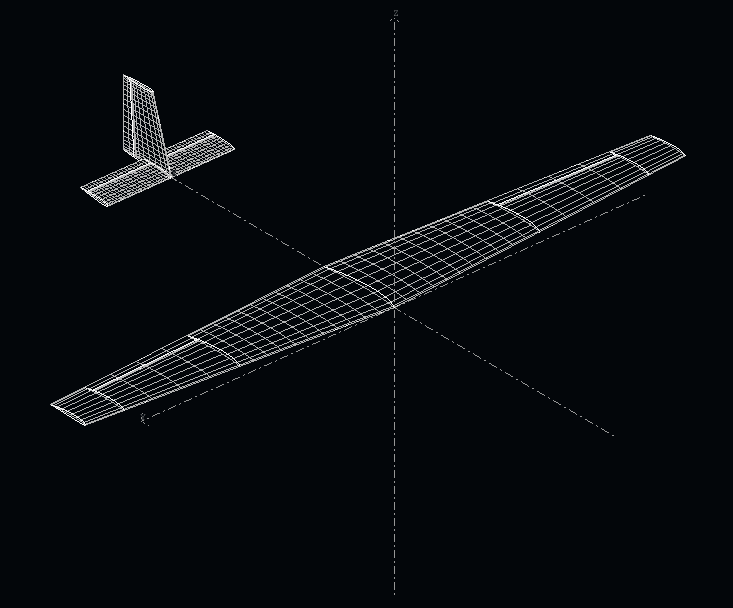
\includegraphics[width=0.7\textwidth]{Figures/PS3/SkynetV3_XFLR_pic.png}
  \caption{VLM model of our design in XFLR5}\label{fig:vlm-design}
\end{figure}

\subsection{Performance Characteristics}
\label{PerfChar}

The different performance parameters of our design as predicted by XFLR5 are shown in Figures~\ref{fig:cl-alpha} to \ref{fig:power-cons}.

\begin{figure}[h!]
  \centering
  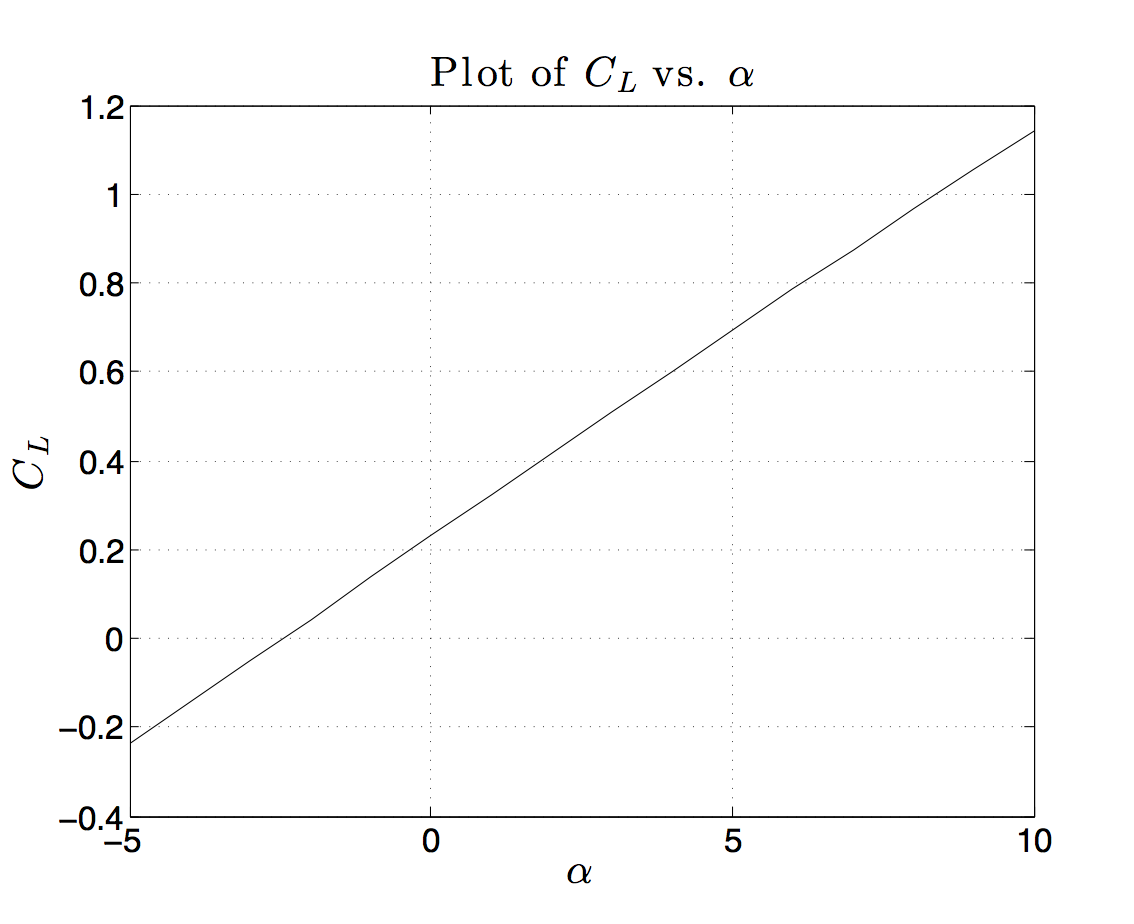
\includegraphics[width=0.7\textwidth]{Figures/PS3/CL_vs_alpha.png}
  \caption{$C_L$ vs $\alpha$}\label{fig:cl-alpha}
\end{figure}
\begin{figure}[h!]
  \centering
  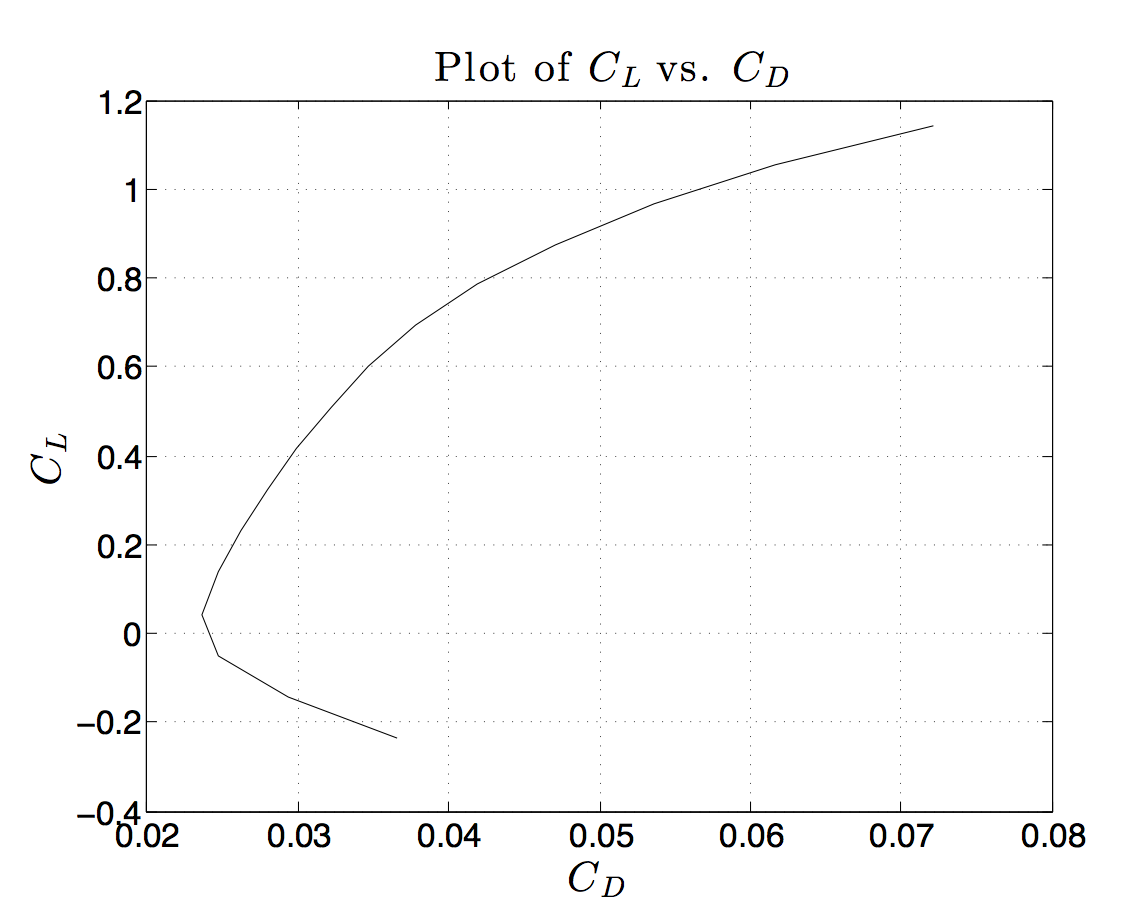
\includegraphics[width=0.7\textwidth]{Figures/PS3/CL_vs_CD.png}
  \caption{Drag polar}\label{fig:cl-cd}
\end{figure}
\begin{figure}[h!]
  \centering
  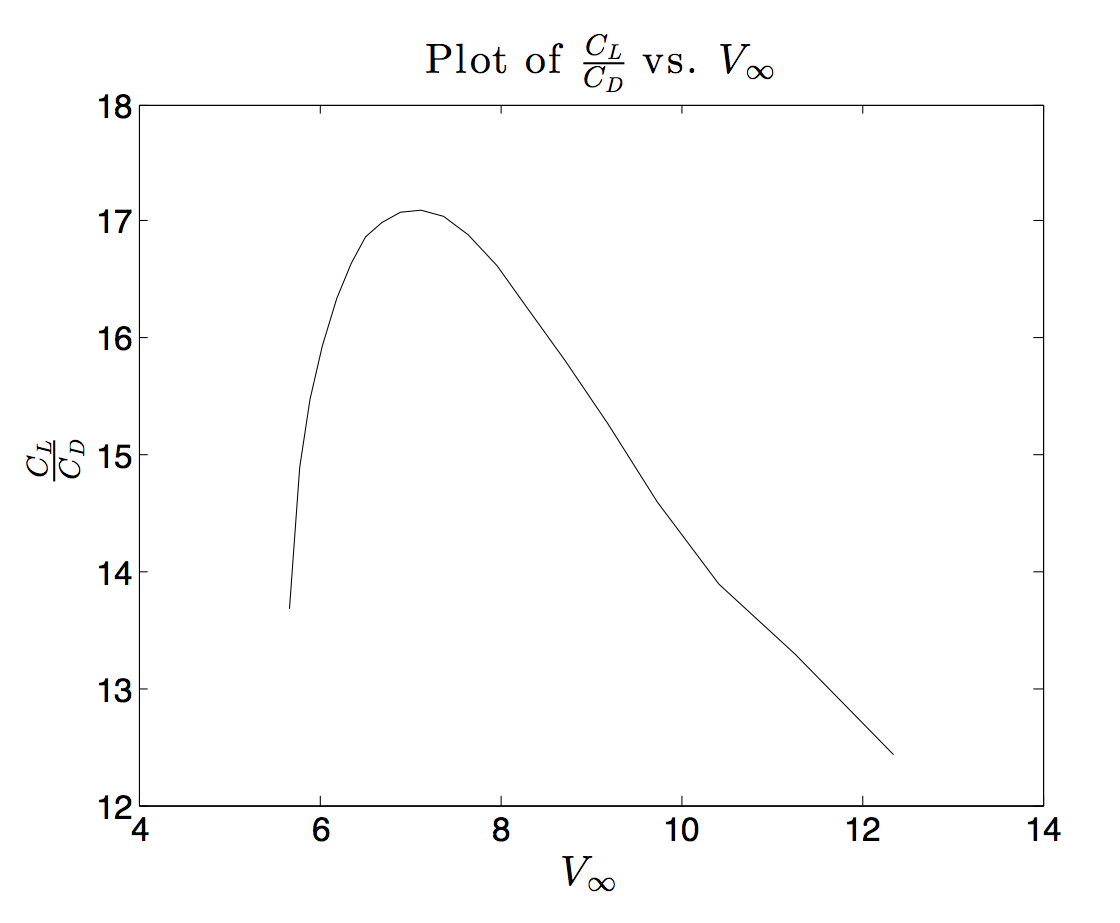
\includegraphics[width=0.7\textwidth]{Figures/PS3/CL-CD_vs_V.png}
  \caption{$C_L/C_D$ vs $v_\infty$}\label{fig:LD-v}
\end{figure}
\begin{figure}[h!]
  \centering
  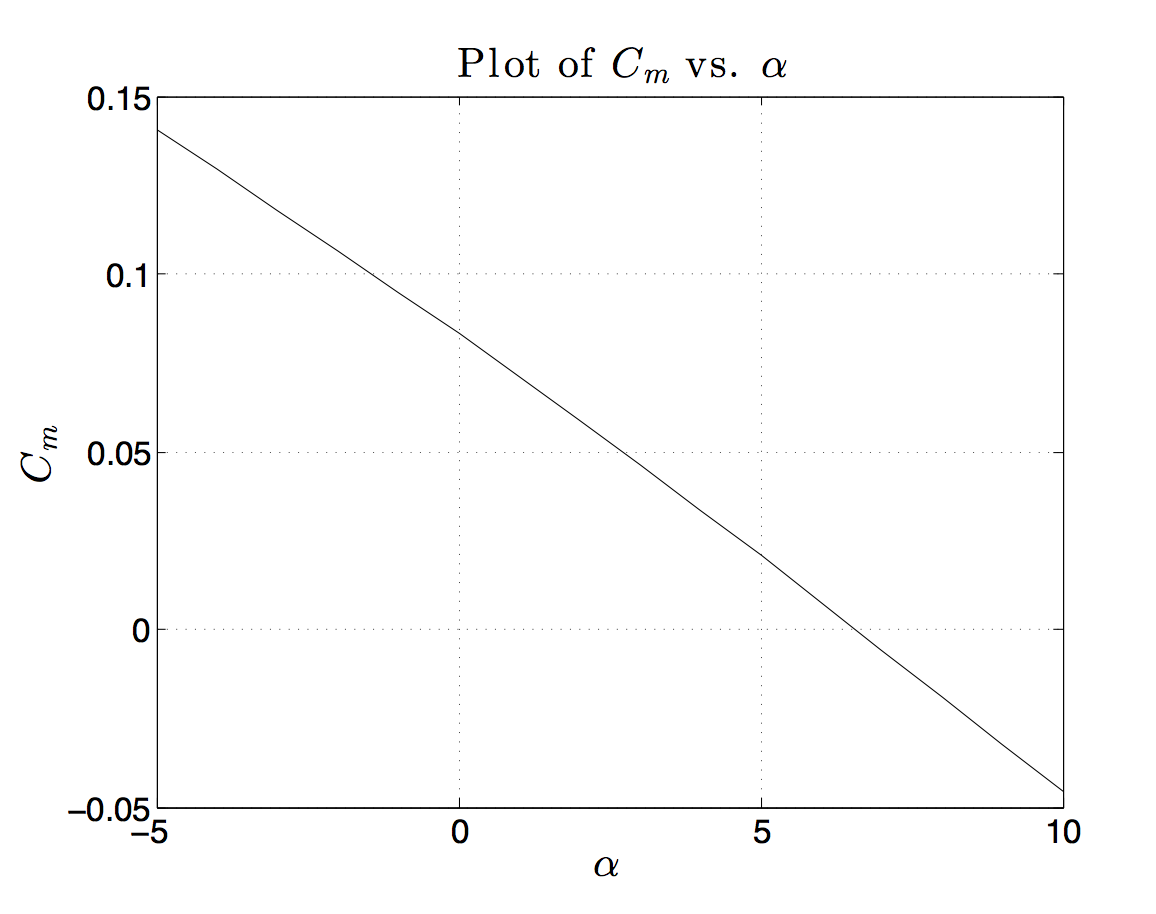
\includegraphics[width=0.7\textwidth]{Figures/PS3/Cm_vs_alpha.png}
  \caption{$C_m$ vs $\alpha$}\label{fig:cm-alpha}
\end{figure}
\begin{figure}[h!]
  \centering
  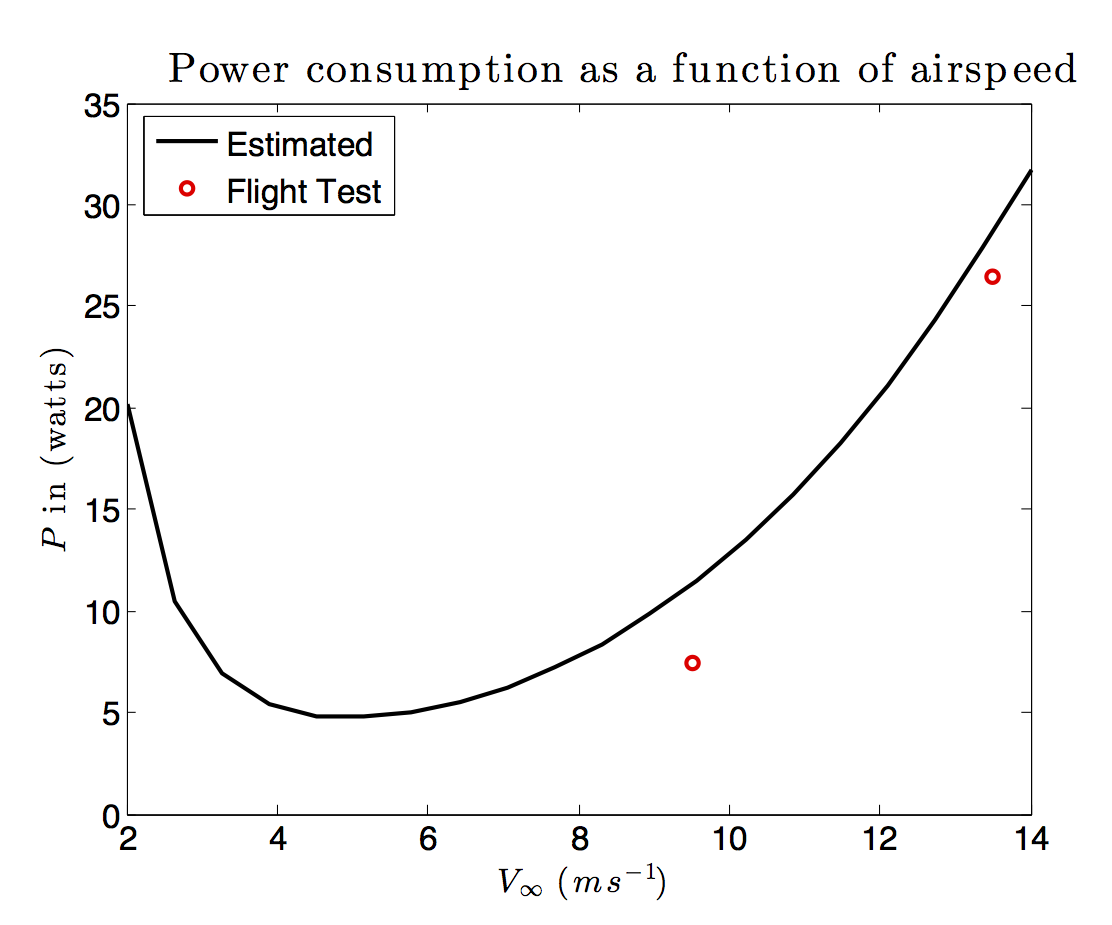
\includegraphics[width=0.7\textwidth]{Figures/PS3/power_consumption.png}
  \caption{$P_{level}$ vs airspeed}\label{fig:power-cons}
\end{figure}

A comparison of the performance parameters estimated from our analysis with the performance parameters obtained from measured data during flight tests in shown in Table~\ref{table:Compar}.

\begin{table}[htb]
\begin{center}
\begin{tabular}{|c|c|c|c|c|c|}
\hline
\textbf{} & \textbf{$C_L\;max$} & \textbf{$(L/D)_{max}$} & \textbf{$P_{level}$ $(9.5 \; ms^{-1})$} & $P_{level}$ $(13.5 \; ms^{-1})$  & \textbf{$P_{max\;climb}$} \\ 
\hline
\textbf{Estimated} & $1.14$ & $19.0$ & $11.29\;watts$ & $28.62\;watts$ & $34.12\;watts$  \\
\textbf{Measured}  & $0.73$ & $16.3$ & $7.45\;watts$ & $26.47\;watts$ & $39.98\;watts$  \\
\hline
\end{tabular}
\end{center}
\caption{Estimated vs. measured flight performance parameters}
\label{table:Compar} 
\end{table}

\subsection{Stability Analysis}

The stability analysis of our design was performed in AVL. Three different straight and level flight trim states and one level turn trim state were analysed. The four cases used are listed in Table~\ref{table:stab-cases}.

\begin{table}[htb]
\begin{center}
\begin{tabular}{|c|c|c|}
\hline
\textbf{Case} & \textbf{Airspeed (in m/s)} & \textbf{Bank Angle (in degrees)} \\ 
\hline
Case 1 &  $8.5$ &  $0$ \\
Case 2 &  $7.0$ &  $0$ \\
Case 3 & $10.0$ &  $0$ \\
Case 4 &  $8.5$ & $30$ \\
\hline
\end{tabular}
\end{center}
\caption{Different cases for stability analysis in AVL}
\label{table:stab-cases} 
\end{table}

The eigenvalues, frequencies and damping ratios for the different modes are plotted in Figures~\ref{fig:eig},~\ref{fig:freq} and \ref{fig:damp}.

\begin{figure}[h!]
  \centering
  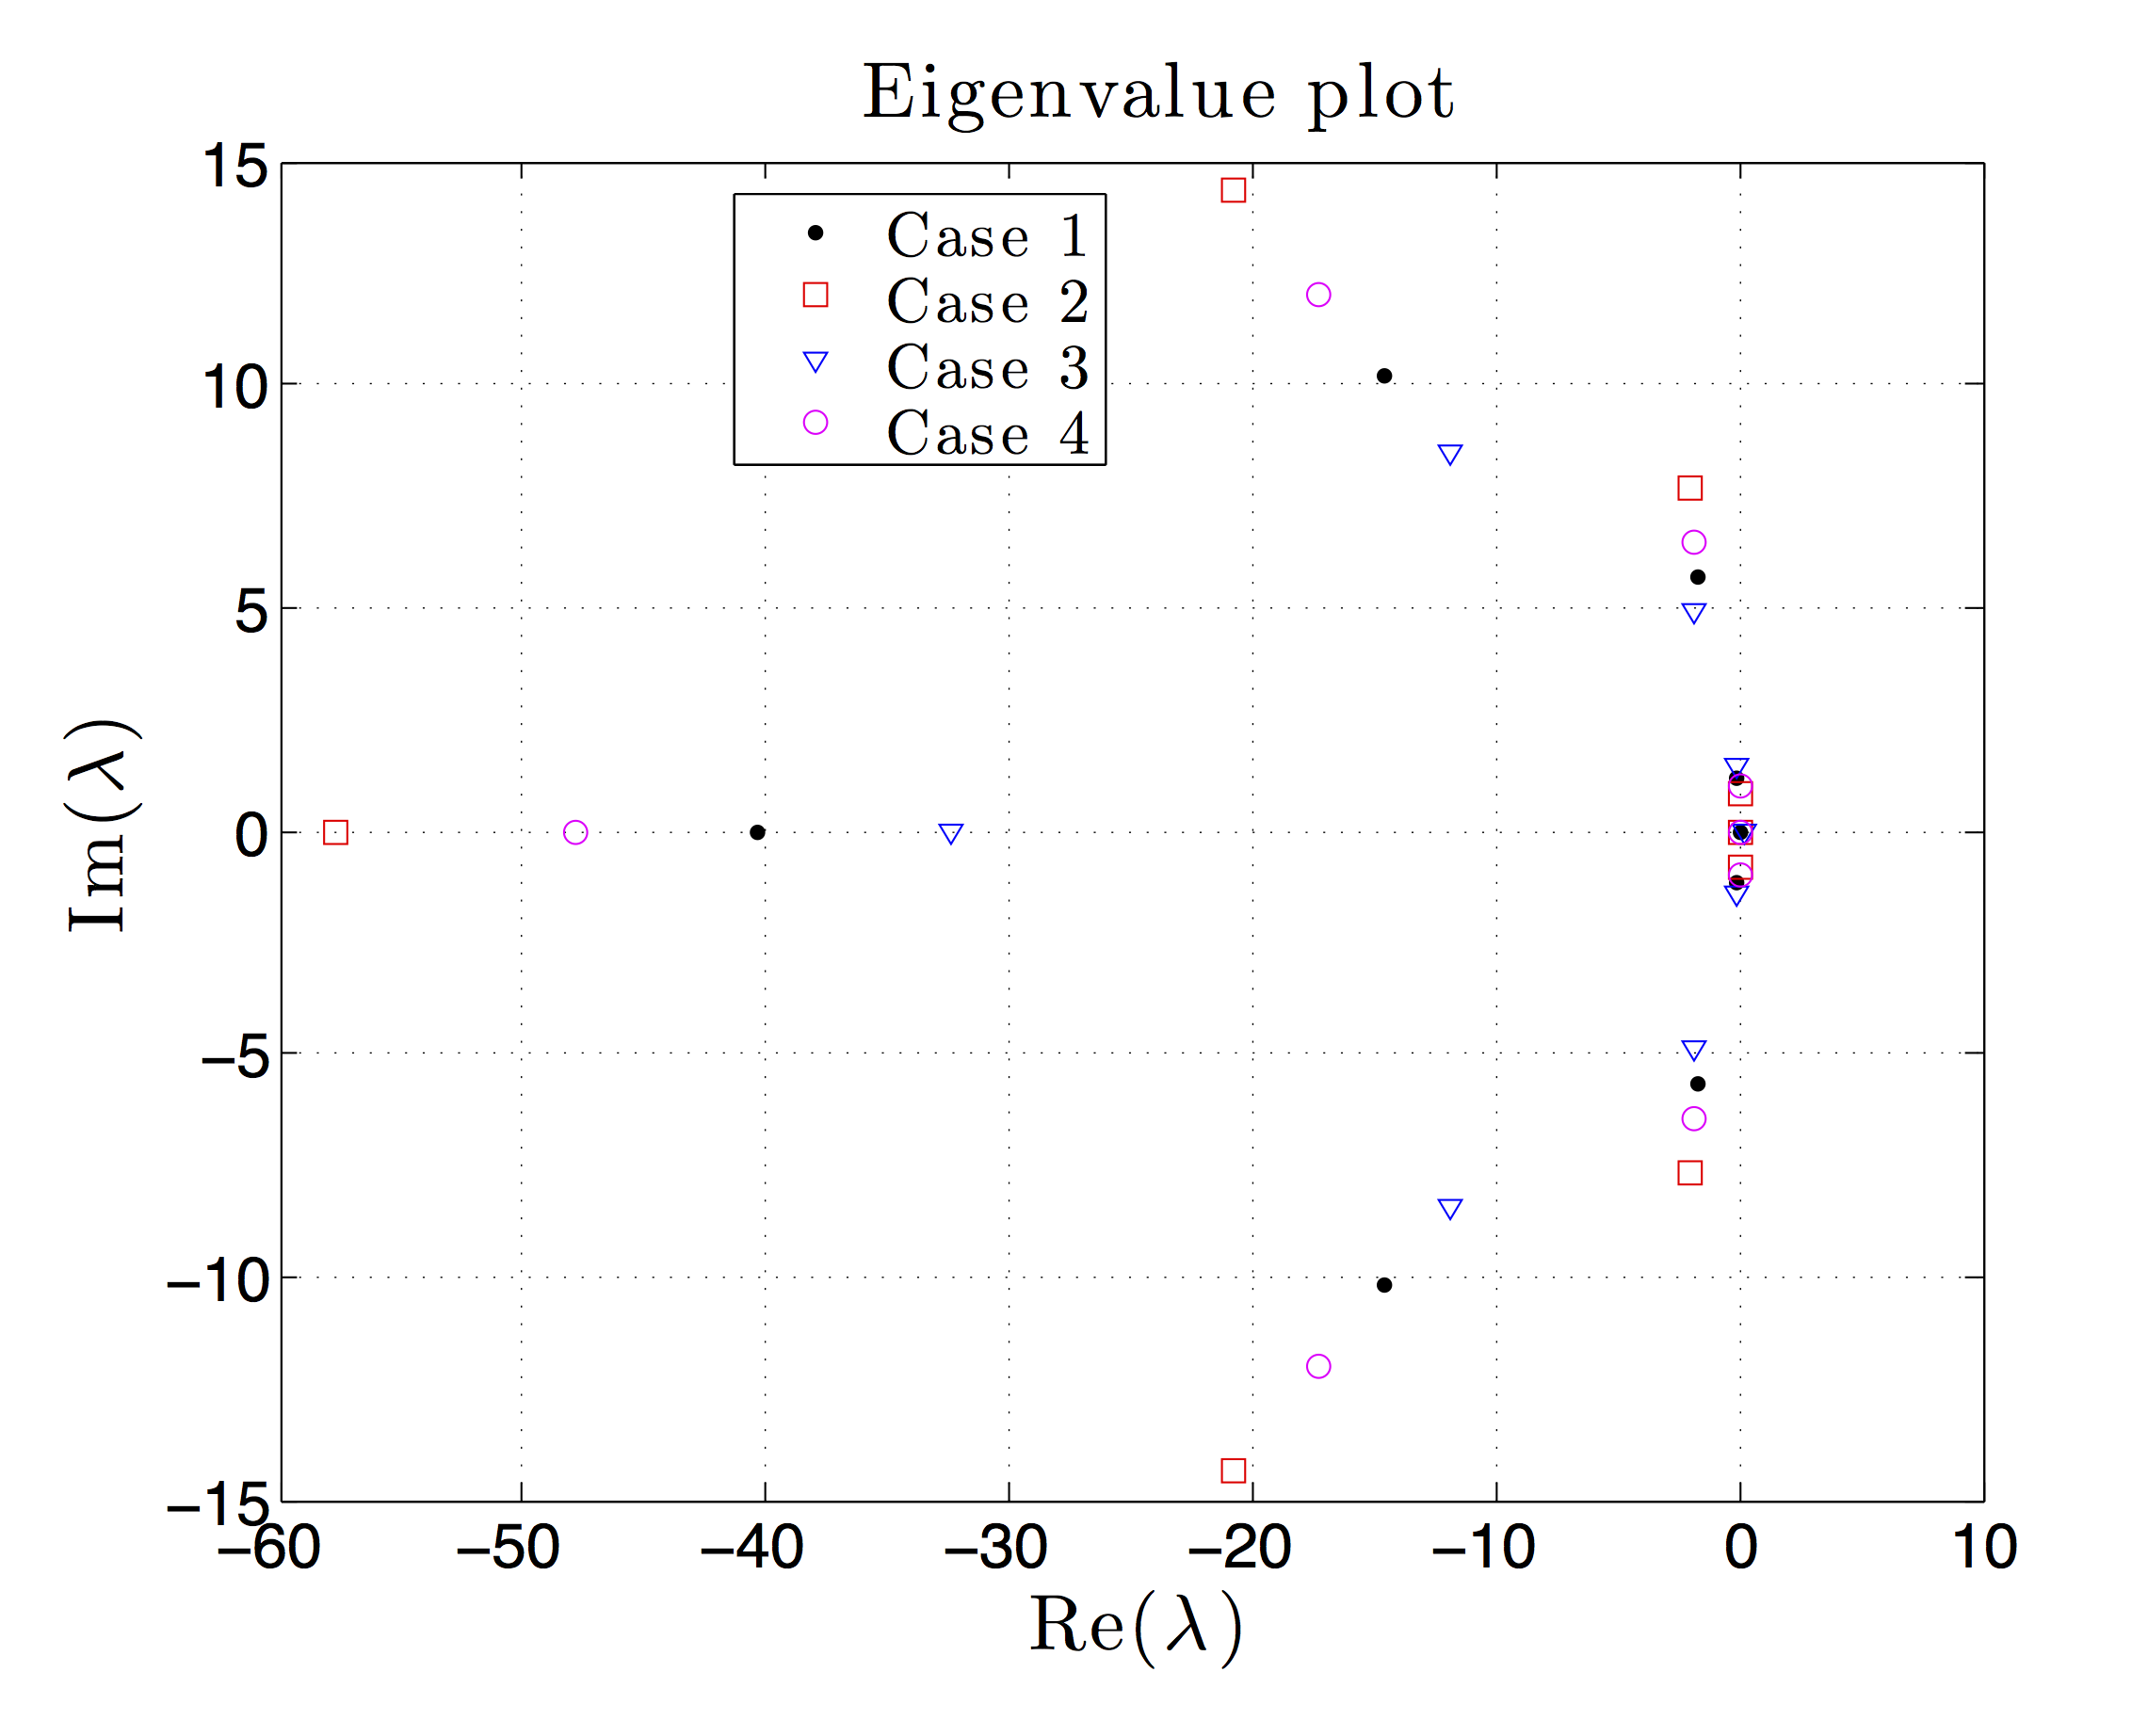
\includegraphics[width=0.7\textwidth]{Figures/PS2/SkynetV1_eig.png}
  \caption{Eigenvalue plot}\label{fig:eig}
\end{figure}
\begin{figure}[h!]
  \centering
  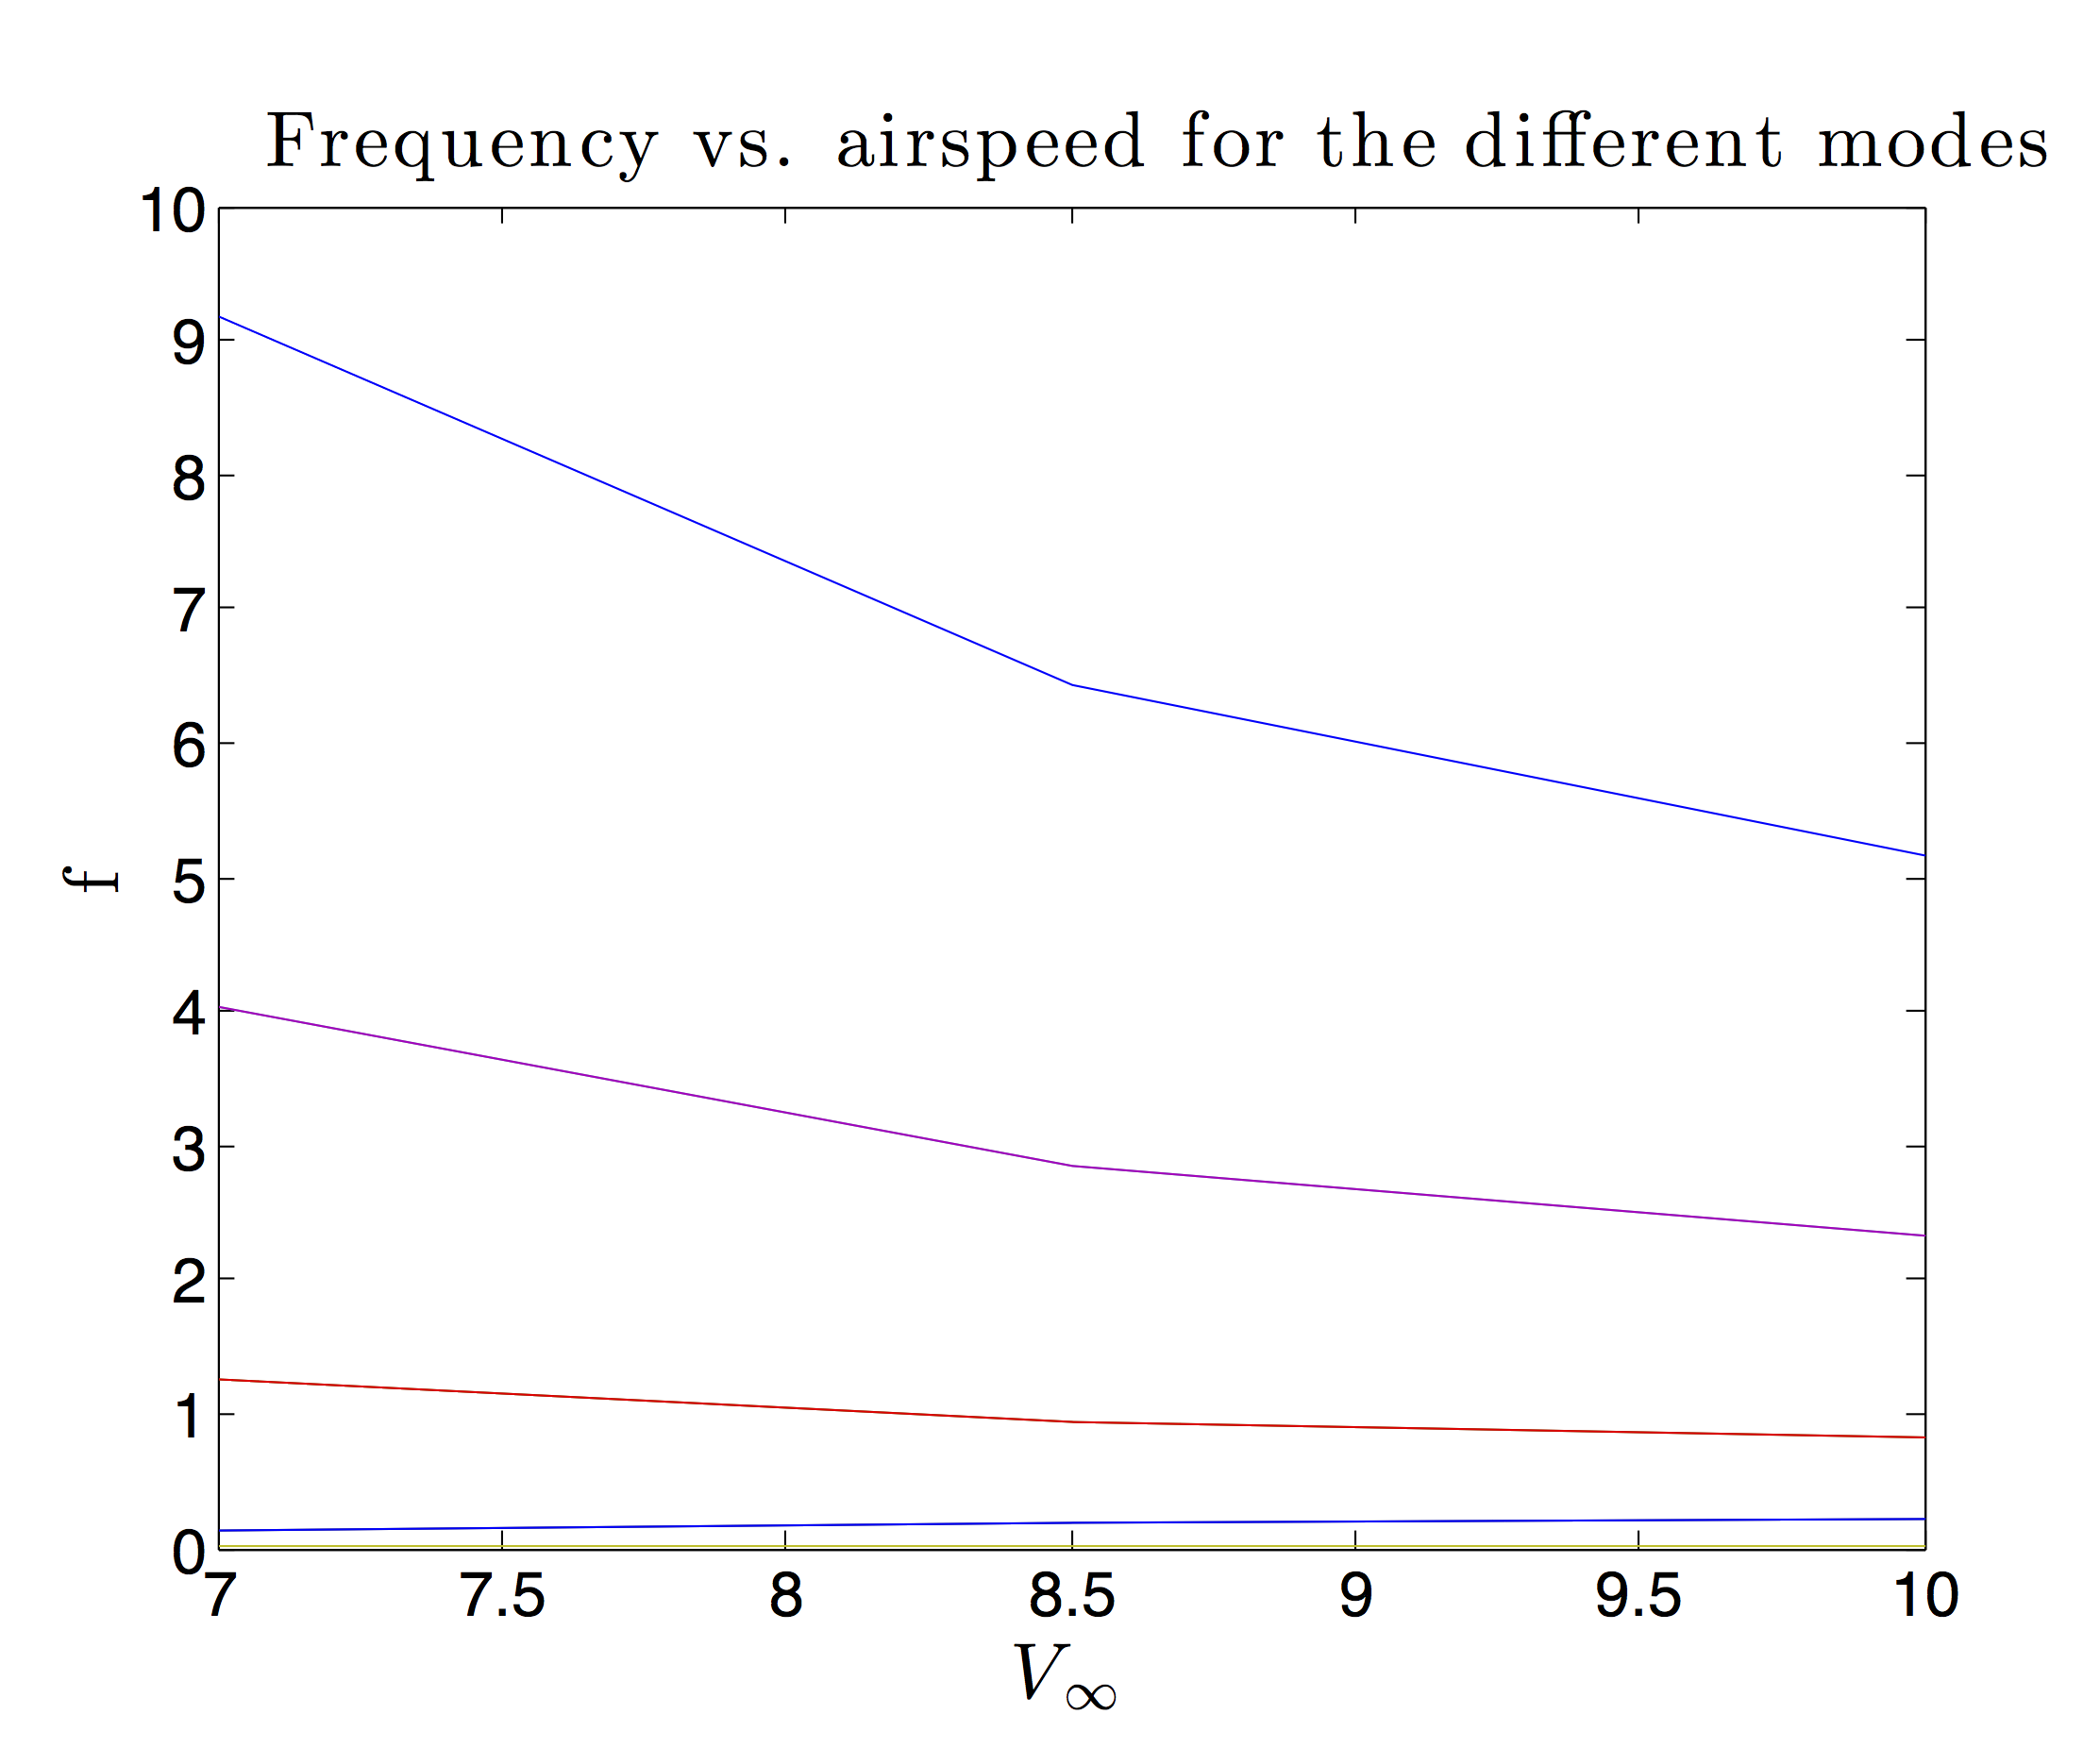
\includegraphics[width=0.7\textwidth]{Figures/PS2/SkynetV1_freq.png}
  \caption{Frequency}\label{fig:freq}
\end{figure}
\begin{figure}[h!]
  \centering
  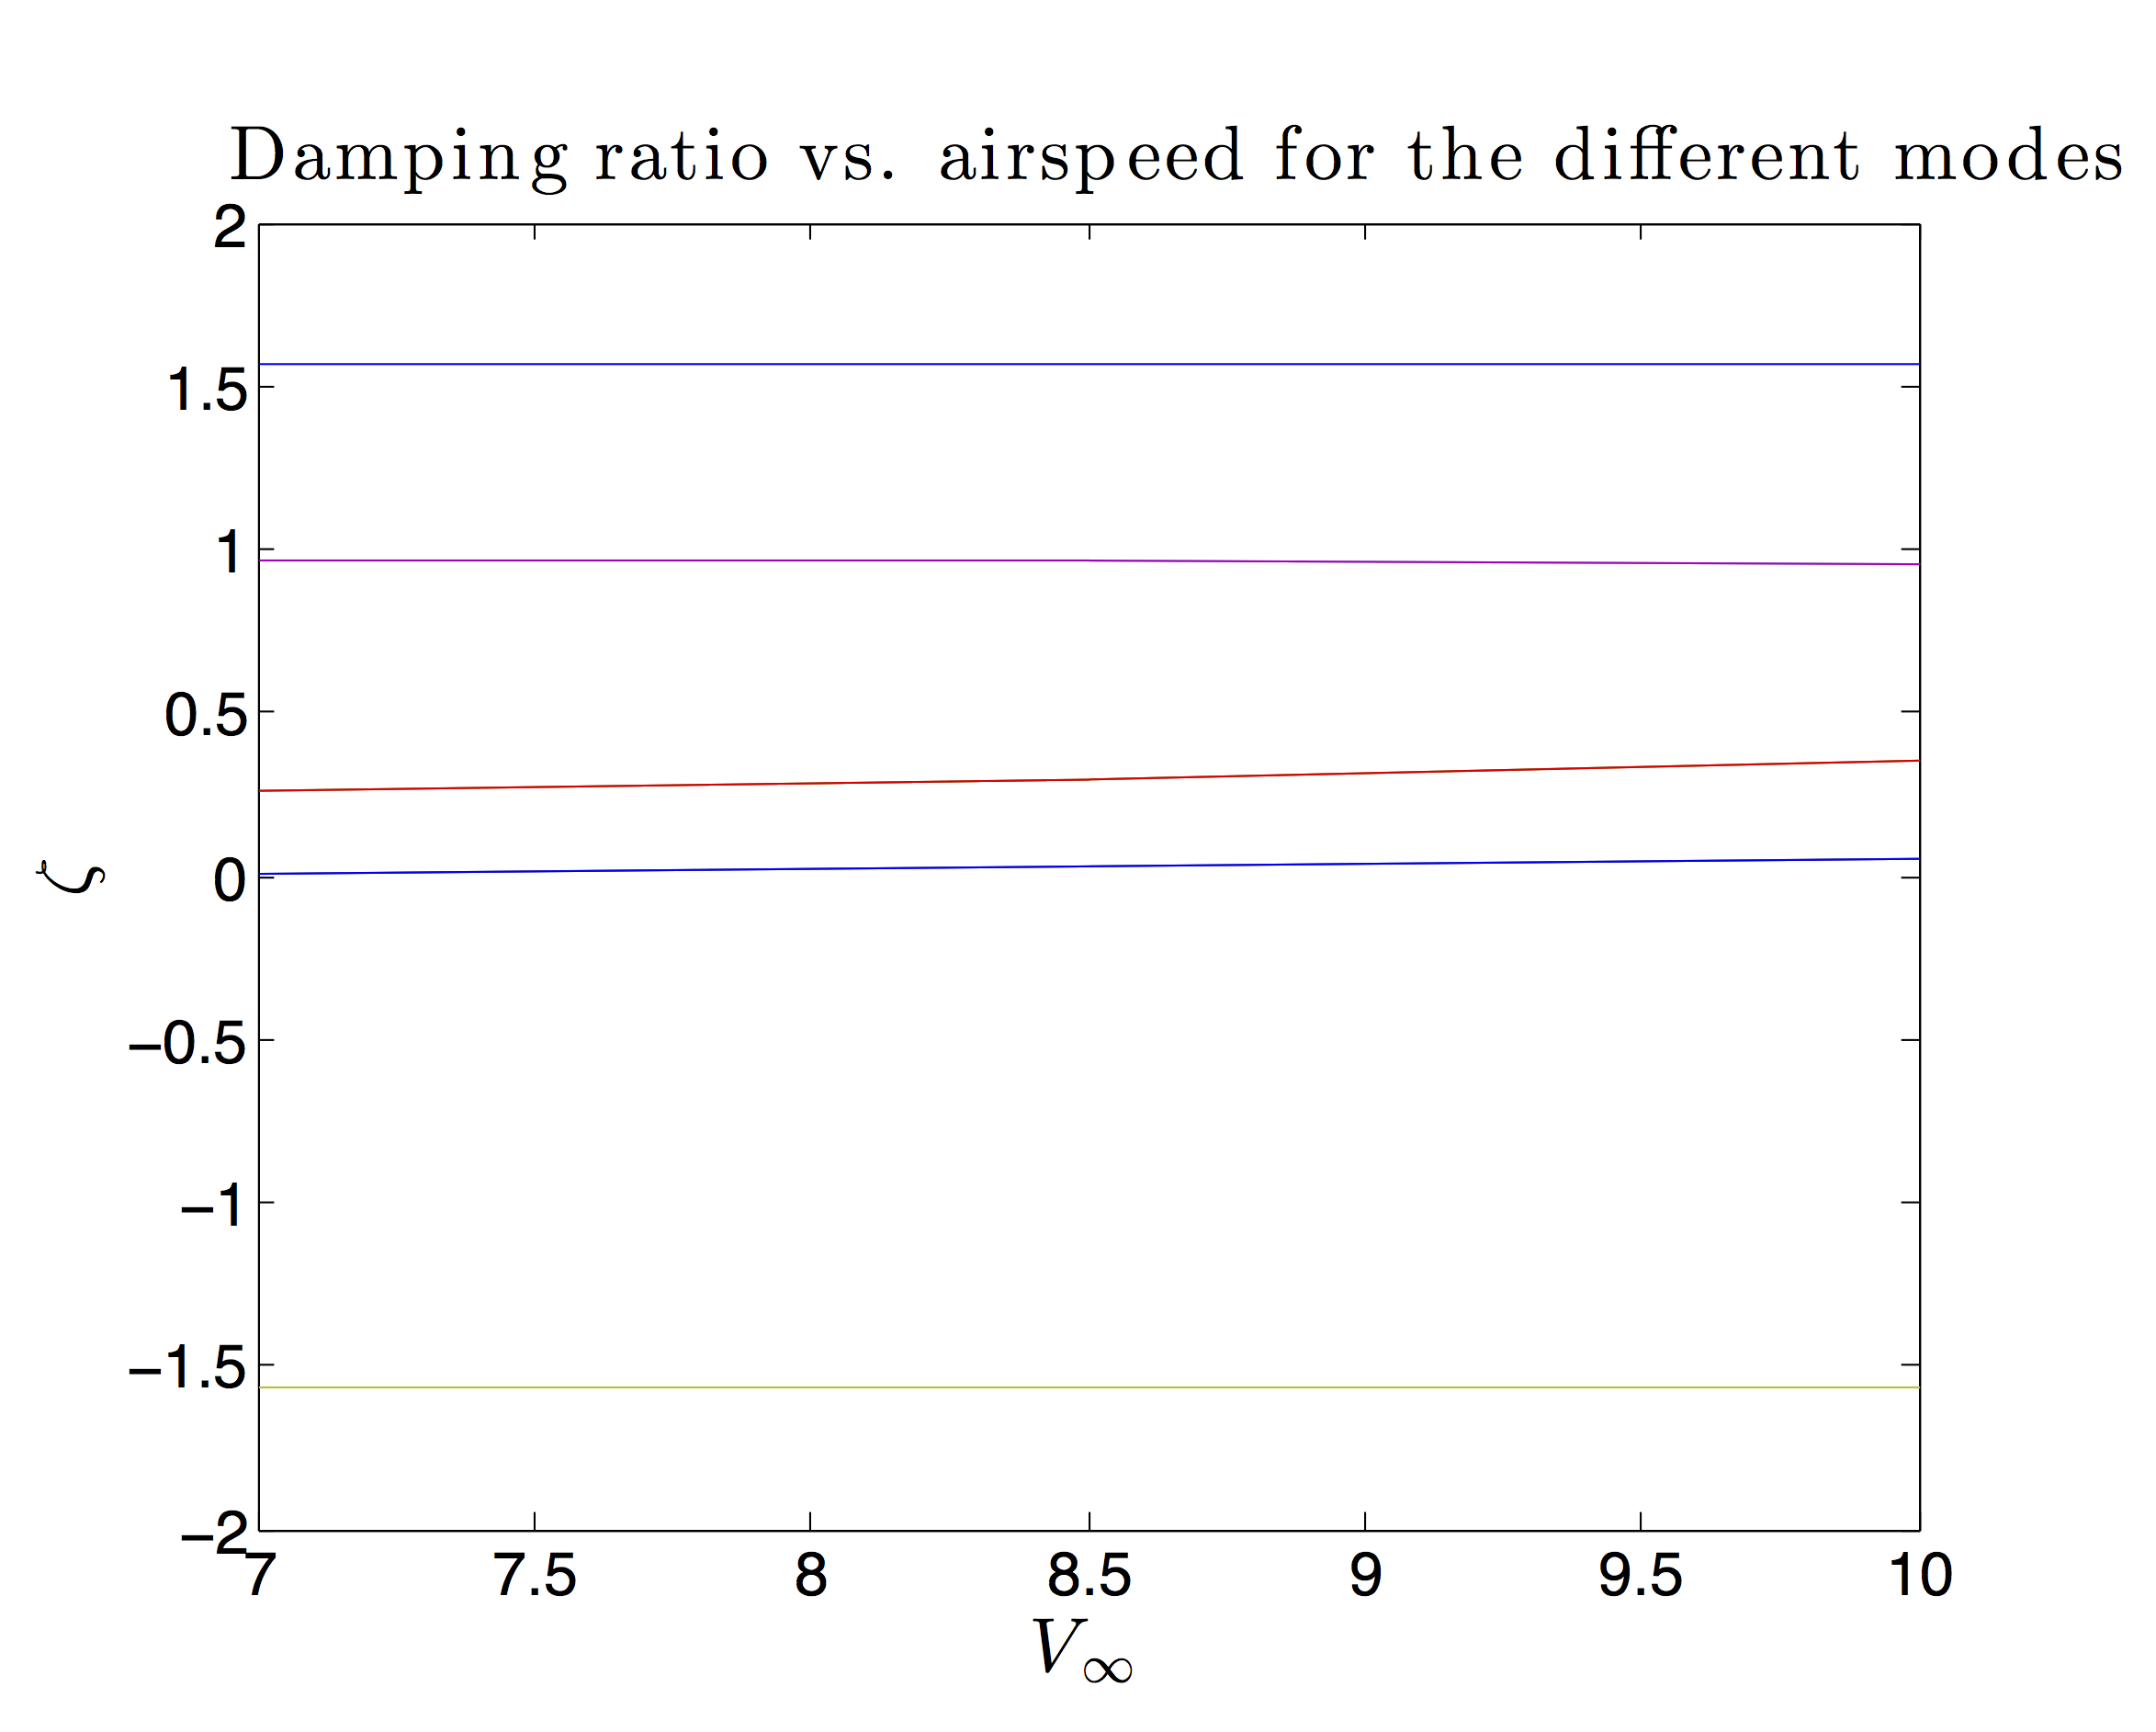
\includegraphics[width=0.7\textwidth]{Figures/PS2/SkynetV1_damp.png}
  \caption{Damping ratio}\label{fig:damp}
\end{figure}

\subsection{Three-view drawings of the final design}

Figure~\ref{fig:CAD} shows the CAD drawings of our final design. Figure~\ref{fig:SW} shows the SolidWorks model of our design that we used to get all the parts for the laser cutter.

\begin{figure}[h!]
  \centering
  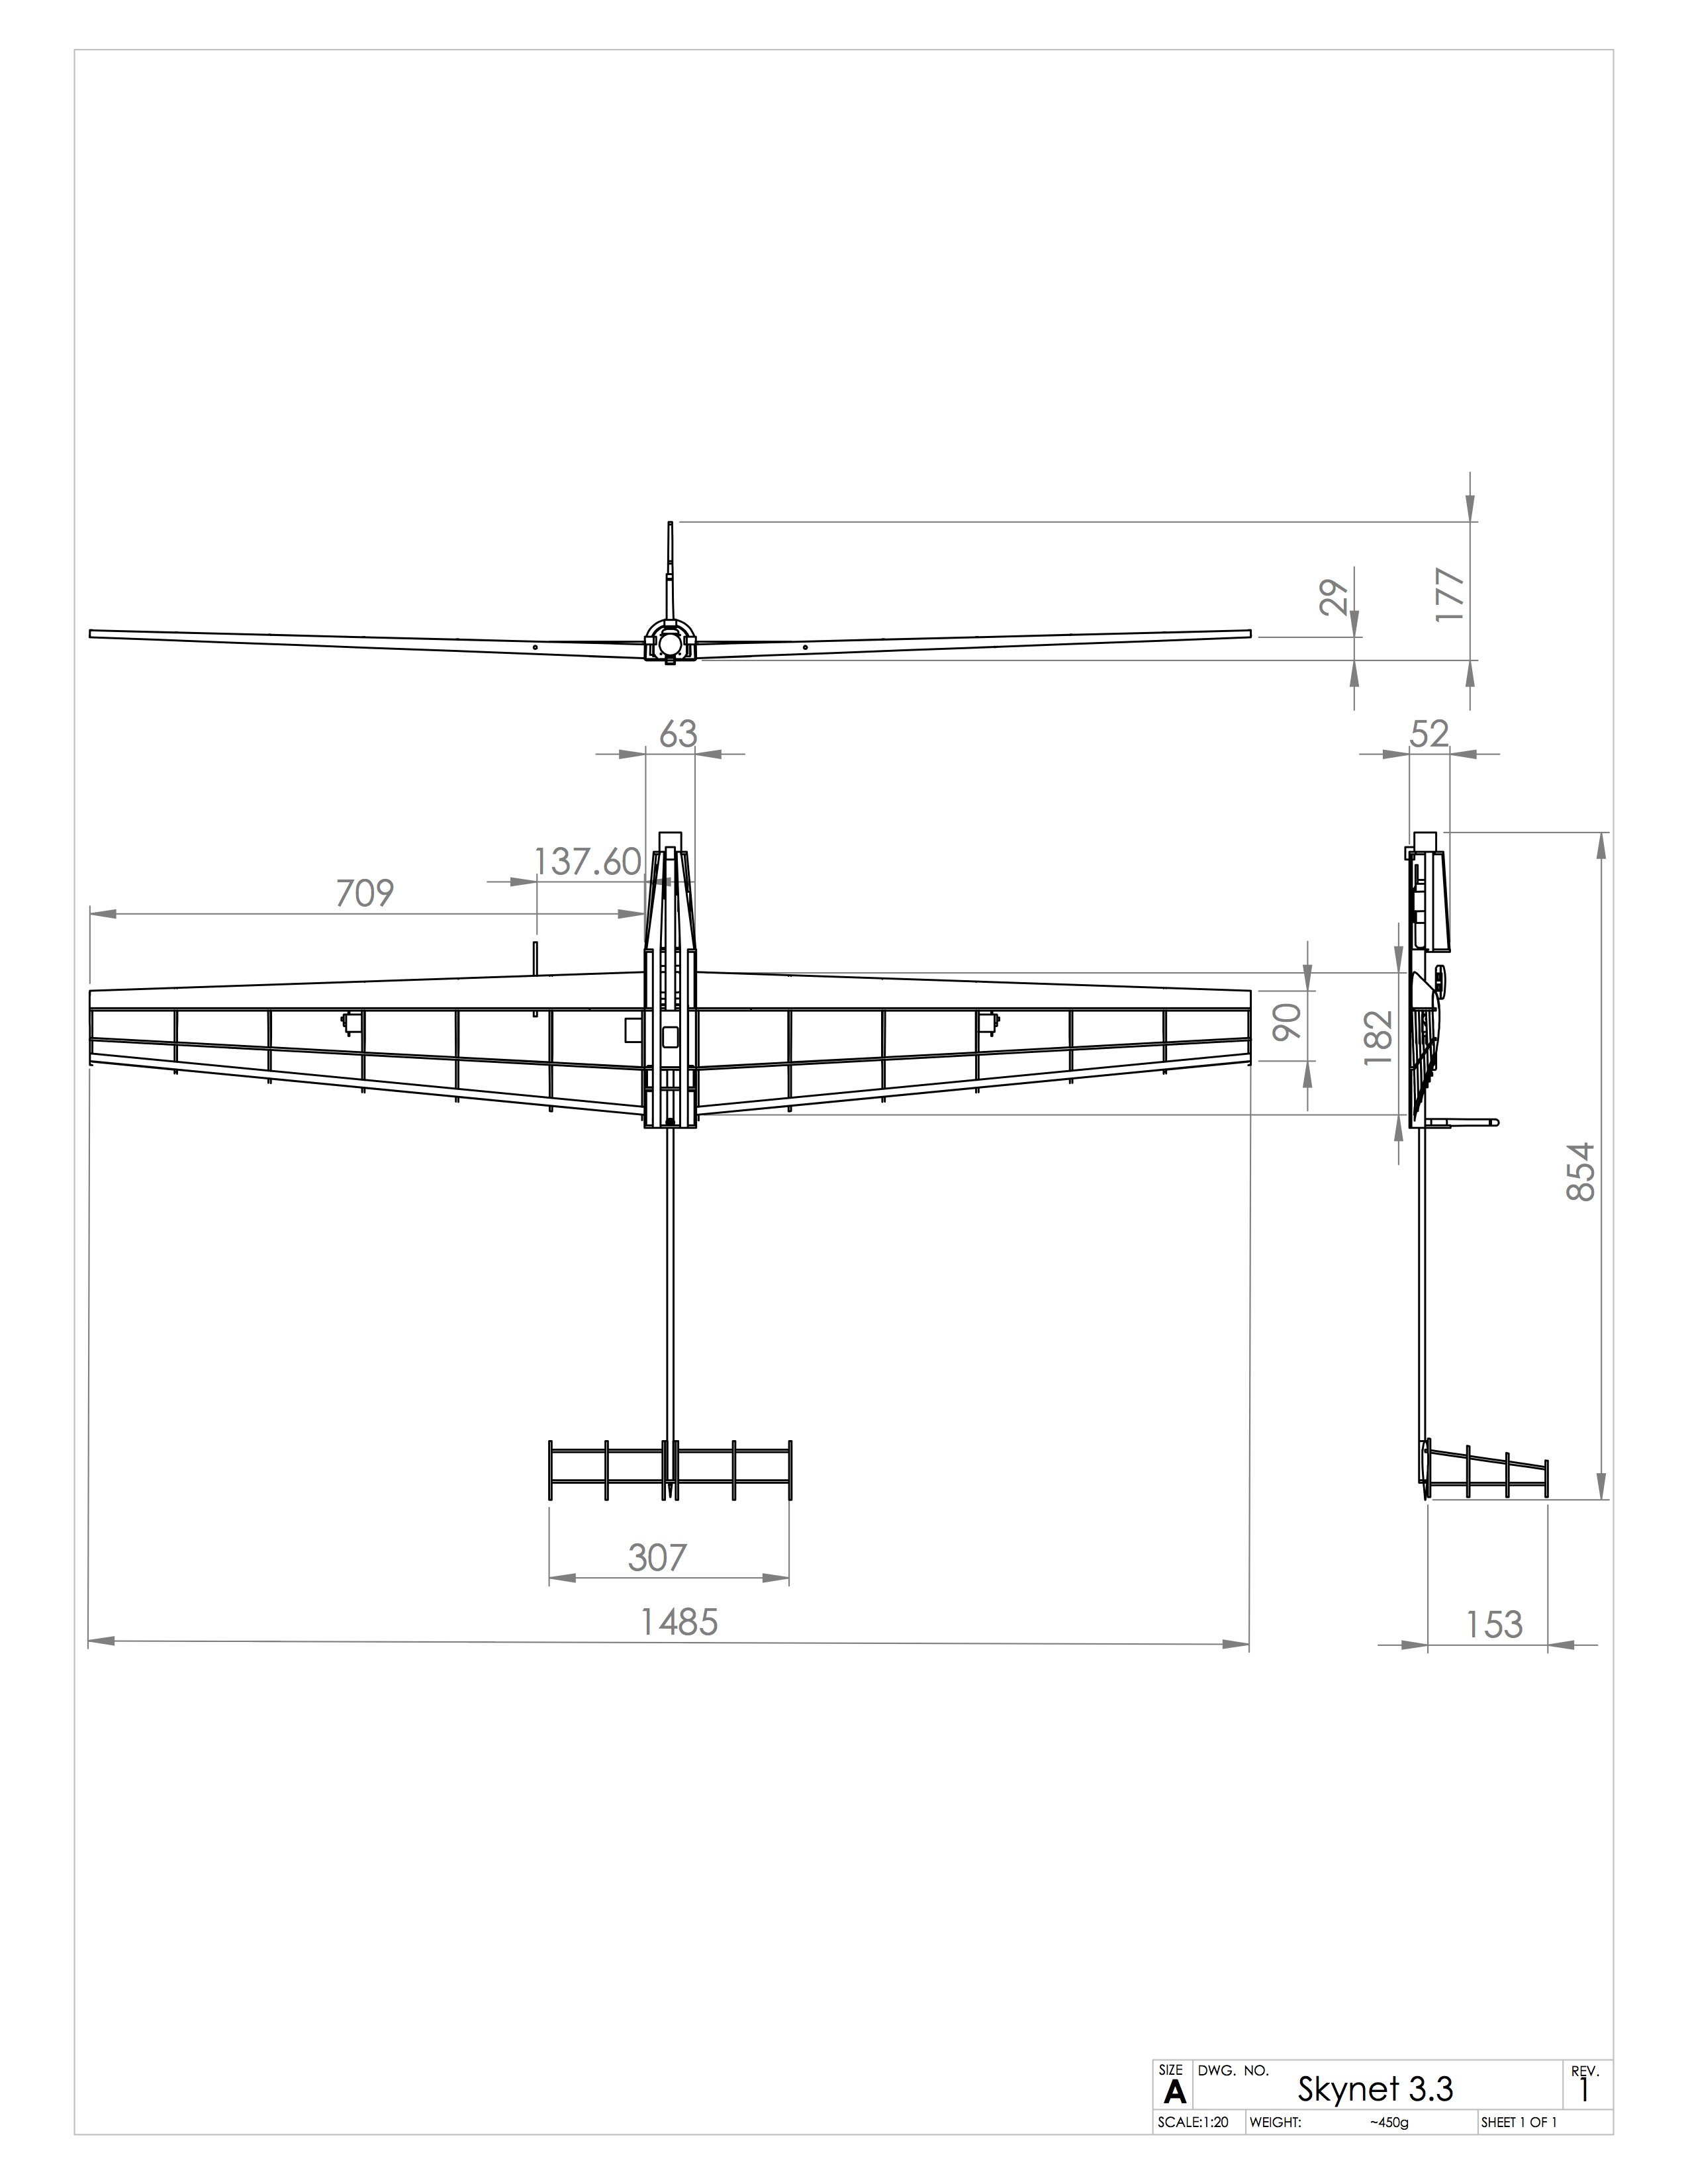
\includegraphics[width=\textwidth]{Figures/CAD/Aircraft_Design_3-3.png}
  \caption{CAD drawings of the final design}\label{fig:CAD}
\end{figure}

\begin{figure}[h!]
  \centering
    \begin{subfigure}[b]{0.49\textwidth}
                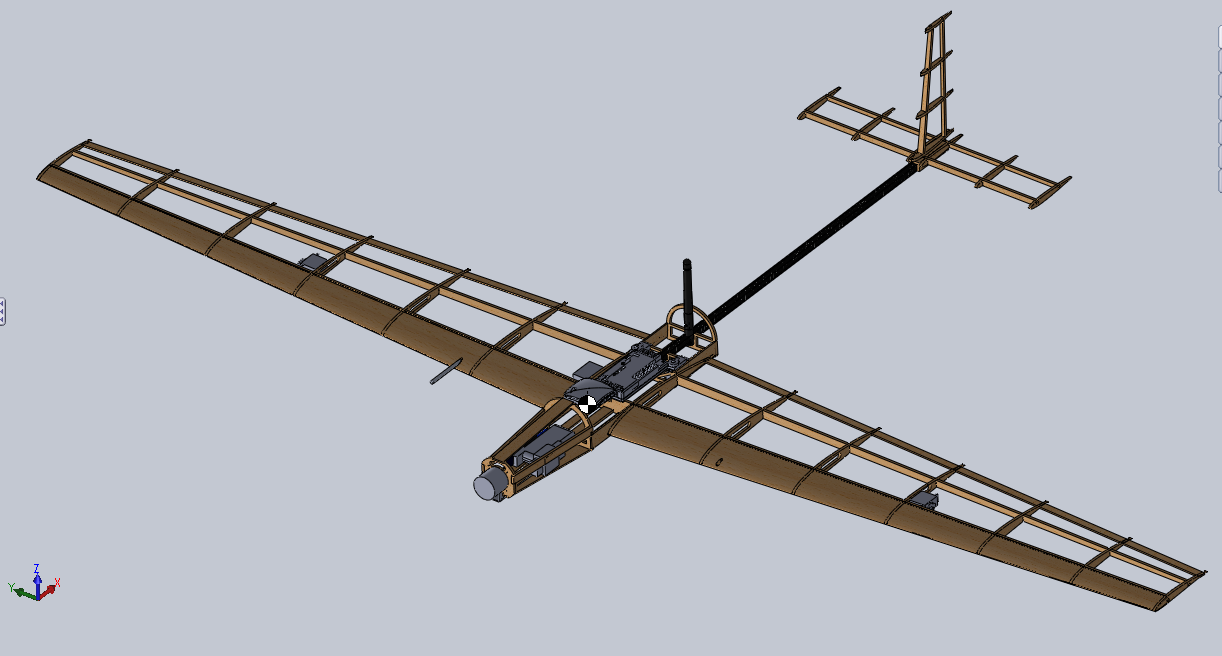
\includegraphics[width=\textwidth]{Figures/CAD/iso.png}
                \caption{Isometric view}
        \end{subfigure}
        \begin{subfigure}[b]{0.49\textwidth}
                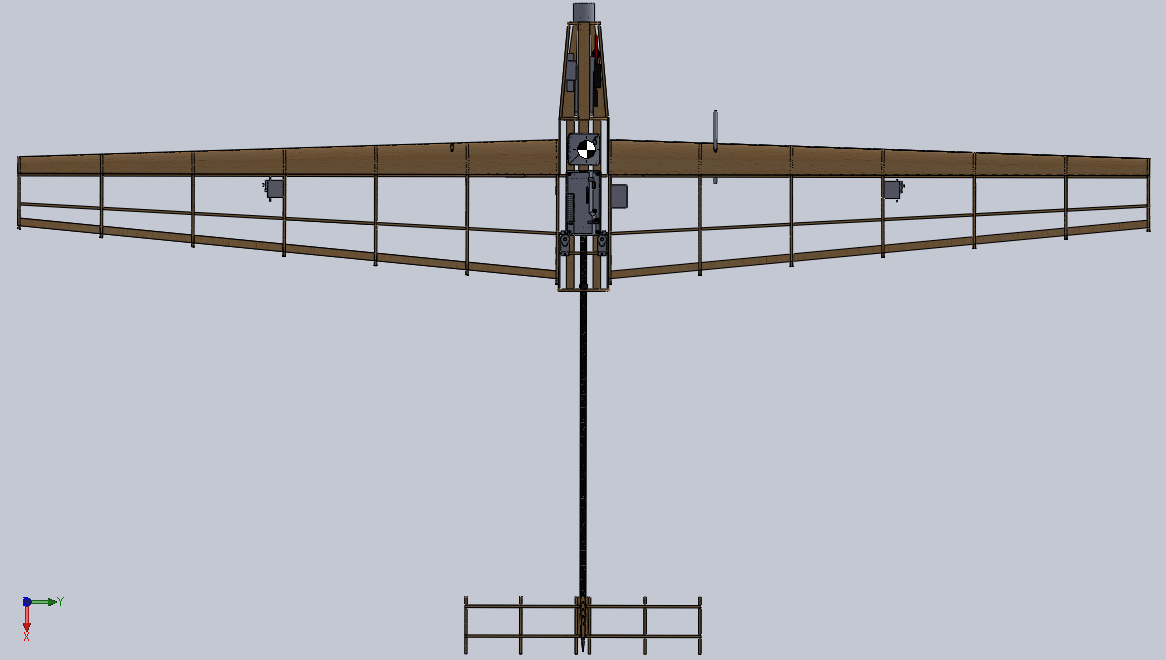
\includegraphics[width=\textwidth]{Figures/CAD/top.png}
                \caption{Top view}
        \end{subfigure}
        \\
        \begin{subfigure}[b]{0.49\textwidth}
                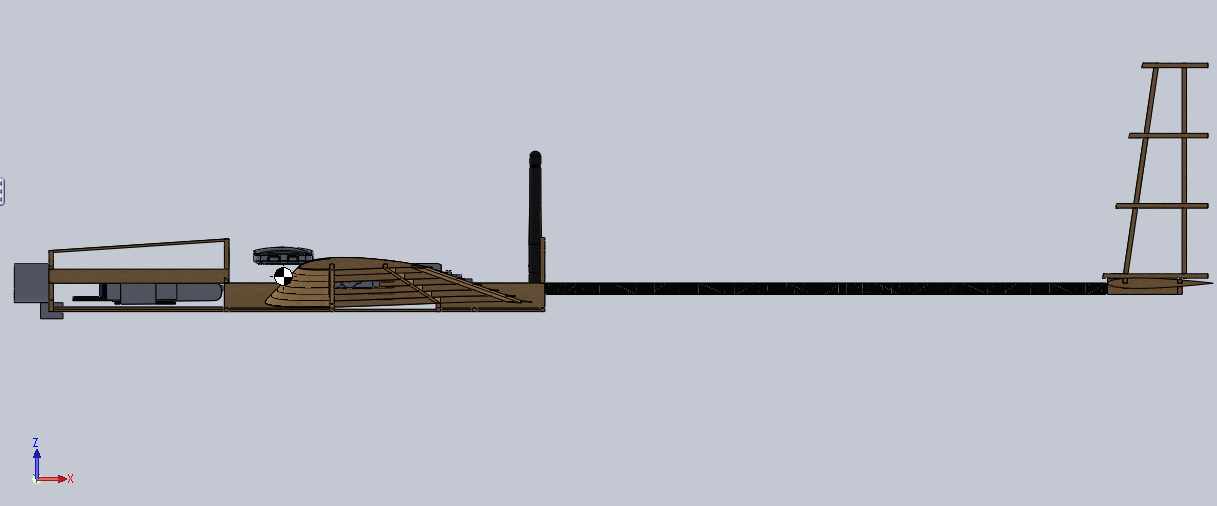
\includegraphics[width=\textwidth]{Figures/CAD/side.png}
                \caption{Side view}
        \end{subfigure}
        \begin{subfigure}[b]{0.49\textwidth}
                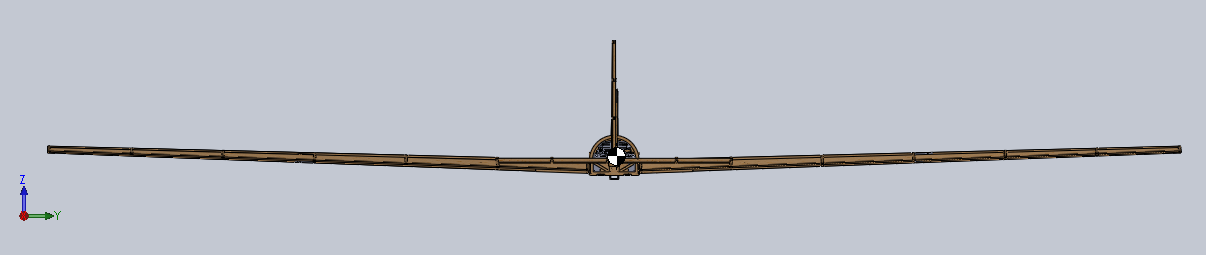
\includegraphics[width=\textwidth]{Figures/CAD/front.png}
                \caption{Front view}
        \end{subfigure}%
  \caption{Solidworks model screenshots}\label{fig:SW}
\end{figure}

% AKSHAY & SRAVYA
% Include in this section a Three View Drawing of the Plane


\section{Controls}
\label{Controls}
\subsection{Control Strategy}
\label{CtrlStr}
\subsection{Flight Performance}
\label{CtrlFlightPerf}
% BRANDON
% Include in this section Initial Approach vs. Final Choices


\section{Fabrication}
\label{Fabrication}
\subsection{Prototype Construction Approach}
\label{ProtoConsAppr}
\subsubsection{Mk-I "The Red Baron"}
\label{mk1}
\subsubsection{Mk-II "The Pig"}
\label{mk2}
\subsubsection{Mk-III.1}
\label{mk3.1}
\subsubsection{Mk-III.2 "Ronald McDonald"}
\label{mk3.2}
\subsubsection{Mk-III.2 "Terminator"}
\label{mk3.3}
\subsubsection{Mk-III.2 "The UltraLight"}
\label{mk3.4}

\section{Flight Testing}
\label{FlightTesting}
\subsection{Flight Test Approach}
\label{FltTstAppr}
\subsection{Simulation vs. Actual Tests}
\label{simvsact}
% JERRY

\section{Mission Flight Results}
\label{MissionFlightResults}
\subsection{Official Flight Results}
\label{OffFltRes}
\begin{center}
    \begin{tabular}{ | c | c | c | c | c | p{3cm} |}
    \hline
    \textbf{Flight} & \textbf{Date} & \textbf{Phase 1} & \textbf{Phase 2} & \textbf{Total} & \textbf{Comments} \\ \hline
    1 & 6/6/2014 &  &  & 76.84 & \\ \hline
    2 & 6/6/2014 &  &  & 50.26 & Dropped\\ \hline
    3 & 6/6/2014 &  &  & 25.27 & Dropped\\ \hline
    4 & 6/6/2014 &  &  & 74.61 & \\ \hline
    5 & 6/6/2014 &  &  & 35.76 & Dropped\\ \hline
    Overall & \multicolumn{5}{c|}{75.725}\\ \hline   
    \end{tabular}
\end{center}

\subsection{Analysis of Flight Data}
\label{AnalFltData}
% JERRY & KARTIKEY
% Include observations about about the validity of our approach.
% What observations from the data might inform future work (beyond the scope of the class).


\section{Conclusions \& Lessons Learned}
\label{Conclusion}
% EVERYONE

\section{Future AA241X Recommendations}
\label{Recommendations}
% EVERYONE

\end{document}